\section{Analysis Strategy}
\label{sec:AnalysisStrategy}
We take different analysis approaches between the below and above 3 TeV signal mass samples. In the analyses below 3 TeV, we adopt the multivariable analyses by training boosted decision tree (BDT) on every mass point. On the other hand, for the mass points above 3 TeV, we adopt the cut-and-counting approach. We describe these strategies below.

\subsection{Analysis strategy below 3 TeV}
\label{subsec:AnaStrategyUnder3TeV}
\subsubsection{Event Selection}
\label{subsubsec:RegionDefUnder3TeV}
In the analysis below 3 TeV signal mass points, one signal region (SR) and one control region (CR) are defined according to the numbers of leptons, top tagged large-$R$ jets, and $b$-tagged small-$R$ jets. 

Figure \ref{fig:EventTopology_Htb} shows the schematic of boosted event topology of an $H^{+}{\rightarrow}tb$ event. A signal event is expected to have one $J_{\text{top-tag}}$, three $b$-jets, and one lepton+MET. However, the $b$-jet originated from the gluon ($b_{4}$ in Figure \ref{fig:FeynmanDiagram_Htb}) is typically not detectable because it tends to fly in the forward directions and outside the detector acceptance. Therefore, at least two $b$-jets are required in this analysis.

Events in the SR are required to have exactly one lepton ($e$ or ${\mu}$) that is matched to the one firing one of the single lepton triggers to be consistent with the signal event, as shown in Figure \ref{fig:EventTopology_Htb}. Events must also have at least one top-tagged large-$R$ jet, at least two small-$R$ jets, and at least two $b$-tagged small-$R$ jets. These small-$R$ jets must additionally satisfy ${\Delta}R(J_{\text{top-tag}}^{1\text{st}}, jet)>1.0$ to ensure these small-$R$ jets are not constituent of the leading top-tagged jet. This analysis does not require missing $E_{T}$. 

The requirements for events in the CR are almost the same as the SR, but only the required number of $b$-tagged small-$R$ jets is different. Exactly one $b$-tagged small-$R$ jet is required in the CR.

After the above selections, the SR and CR are enriched in $t\bar{t}+\text{heavy flavour jets (HF)}$ (i.e., $t\bar{t}+\geq1b$, $t\bar{t}+\geq1c$) and $t\bar{t}+\text{light}$ events, respectively. Therefore, these regions are used to control $t\bar{t}+\text{jets}$ in the final fittings. 

%--- Figure of Event Topology
\begin{figure}[H]
  \centering
  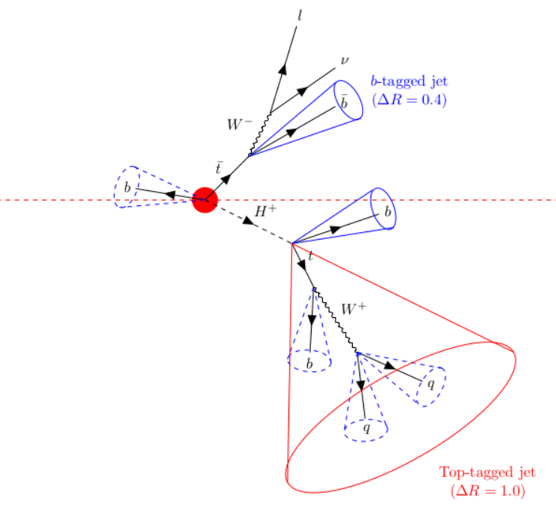
\includegraphics[keepaspectratio,scale=0.8]{images/AnalysisStrategy/EventTopology.png}
  \caption{Schematic of boosted event topology. Signal event has one $J_{\text{top-tag}}$ and at least two $b$-tagged small-$R$ jets.}
  \label{fig:EventTopology_Htb}
\end{figure}
%---

%--- Table of SR1 Event Selections
\begin{table}[H]
  \centering
  \begin{tabular*}{160mm}{l|ll|l}
    \hline\hline
    Cut                       & SR                                                          &                           & CR\\
    \hline
    leptons                   &  - $\text{N}_{\text{lepton}}=1$                             &                           & \\
                              & \underline{Electron}                                        & \underline{Muon}          & Same as SR\\
                              &  - $p_{\text{T}}>27$ GeV                                    &  - $p_{\text{T}}>27$ GeV  & \\
                              &  - $|\eta|<1.37$ or $1.52<|\eta|<2.47$                      &  - $|\eta|<2.5$           & \\
    \hline
    Top-tagged large-$R$ jets &  - $\text{N}_{J_{\text{top-tag}}} \geq 1$                   &                           &\\
                              &  - $350~\text{GeV}<p_{\text{T}}<2500~\text{GeV}$            &                           & Same as SR\\
                              &  - $m>40\text{GeV}$                                         &                           & \\
    \hline
    Small-$R$ jets            &  - $\text{N}_{\text{jet}} \geq 2$                           &                           & $\text{N}_{\text{jet}} \geq 1$ \\
                              &  - $p_{\text{T}}>25$ GeV                                    &                           & (Kinematic requirements\\
                              &  - $|\eta|<2.5$                                             &                           &  are same as SR)\\
                              &  - ${\Delta}R(J_{\text{top-tag}}^{1st}, jet)>1.0$           &                           & \\
    \hline
    $b$-tagged small-$R$ jets & $\text{N}_{b-\text{jet}} \geq 2$                            &                        & $\text{N}_{b-\text{jet}}=1$\\

    \hline\hline
  \end{tabular*}
  \caption{Event selections in the SR and CR. After these selections, the SR becomes enriched in $t\bar{t}+\text{HF}$, and the CR becomes enriched in $t\bar{t}+\text{light}$}
  \label{tab:EventSelectionInSR1AndSR2}
\end{table}

%--- Figure for SR1
\begin{figure}[H]
  \centering
  \subfloat[]{
    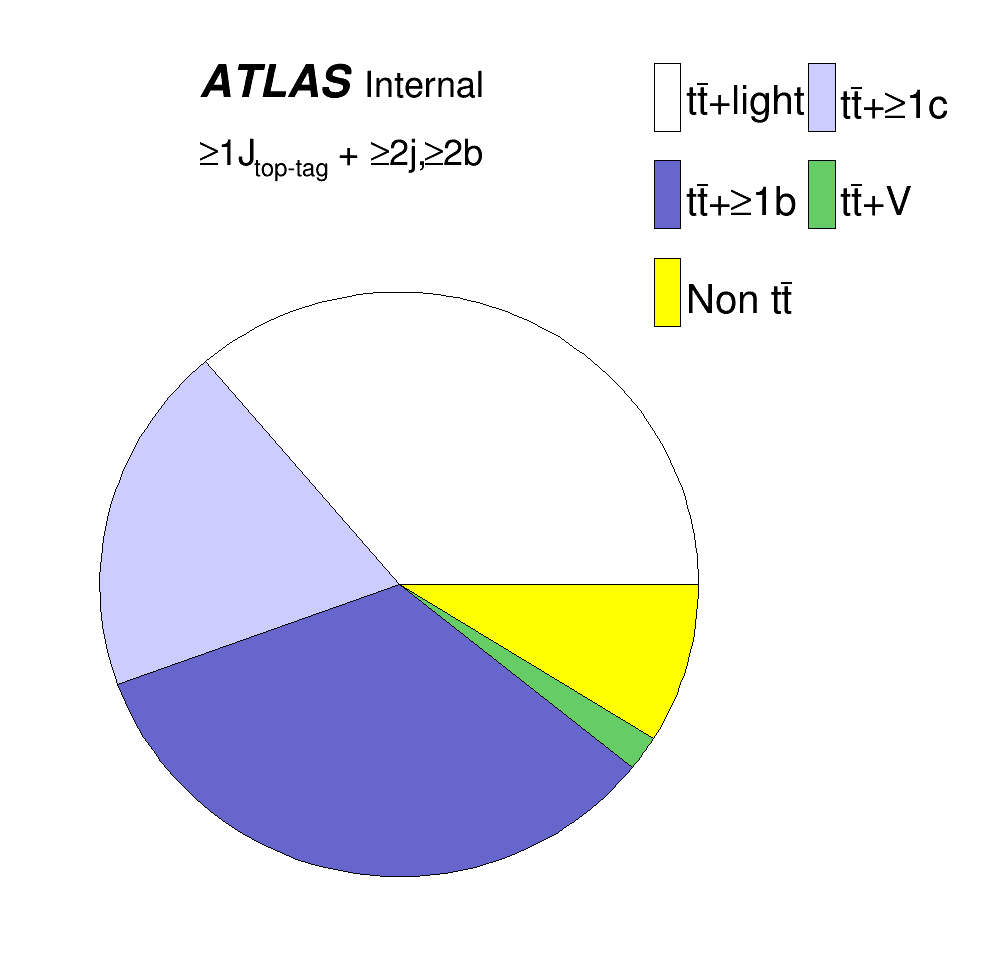
\includegraphics[keepaspectratio,scale=0.2]{images/AnalysisStrategy/PieChart_SR_MVA.png}
    \label{fig:PieChart_SR}
  }
  \subfloat[]{
    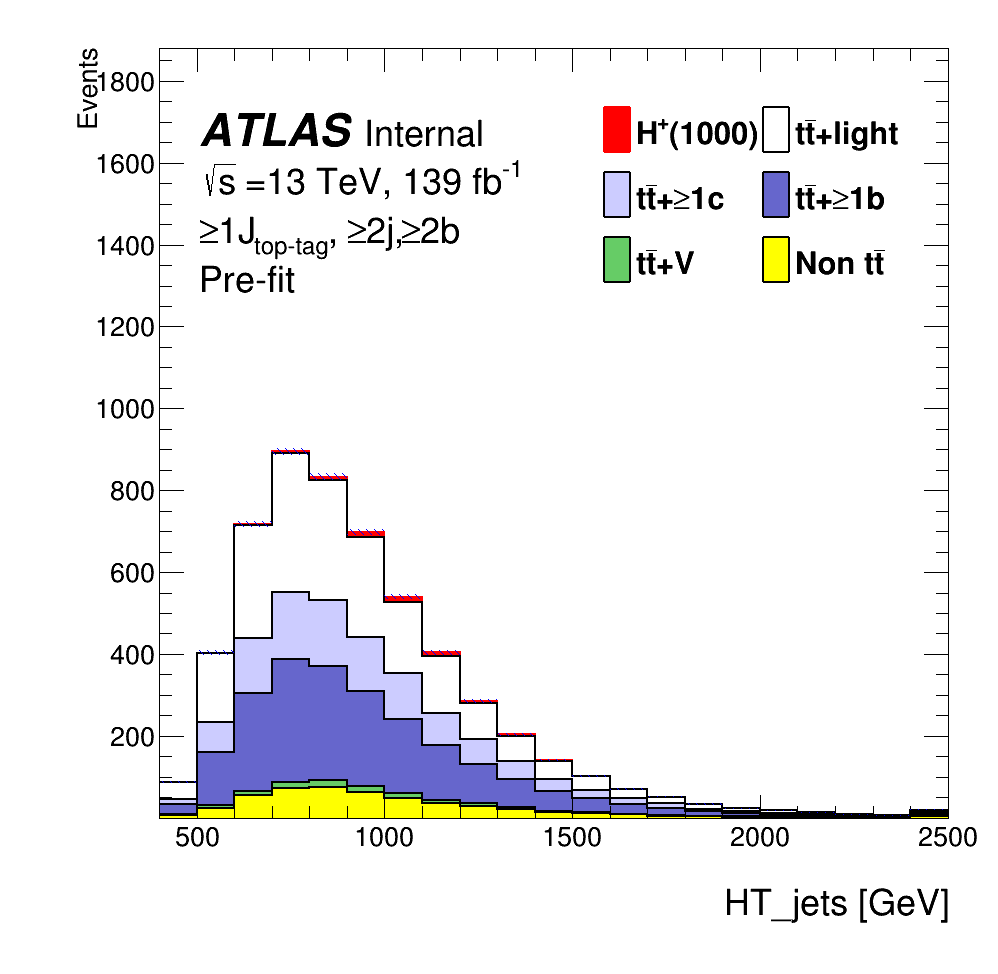
\includegraphics[keepaspectratio,scale=0.2]{images/AnalysisStrategy/HT_jets_SR_MVA.png}
    \label{fig:PieChart_SR1}
  }
  \caption{Background composition in the SR is shown in the pie chart (a) and the $H_{\text{T}}^{\text{jets}}$ distributions (b).}
  \label{fig:BkgComposition_SR1}
\end{figure}


%--- Figure for SR2
\begin{figure}[H]
  \centering
  \subfloat[]{
    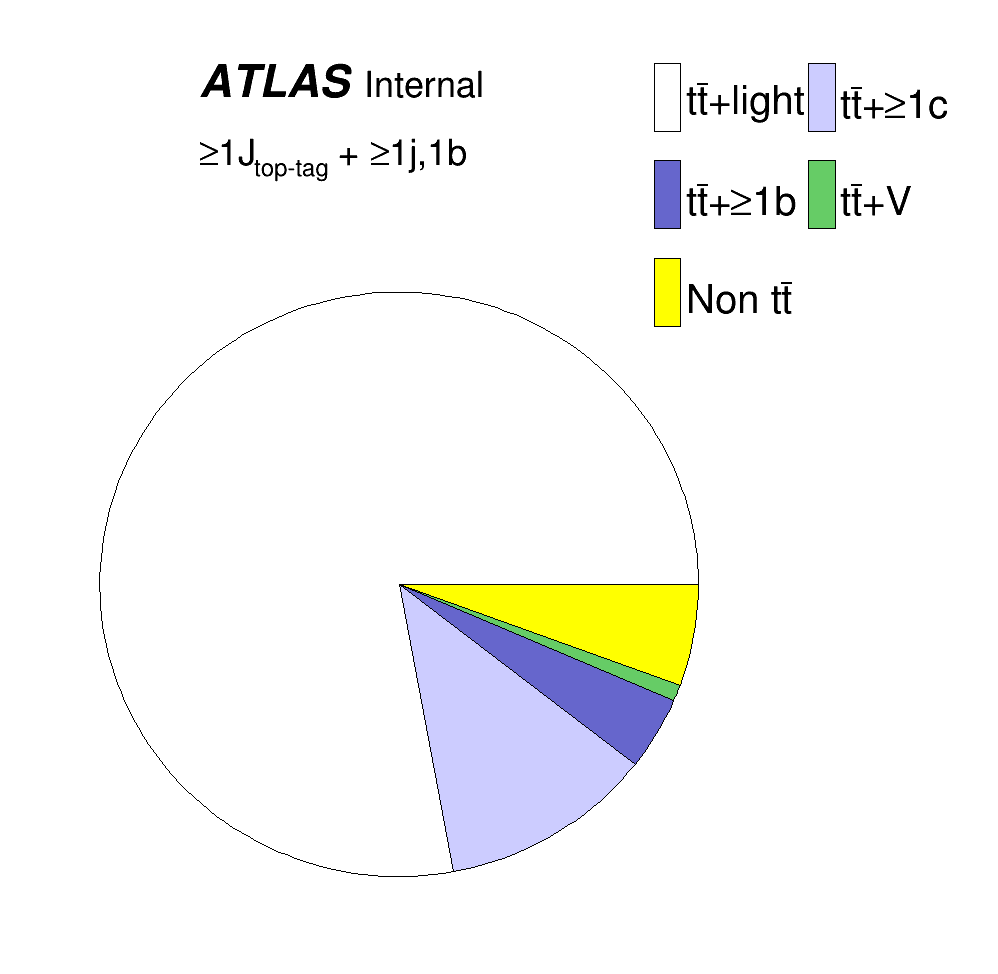
\includegraphics[keepaspectratio,scale=0.2]{images/AnalysisStrategy/PieChart_CR_MVA.png}
    \label{fig:PieChart_SR}
  }
  \subfloat[]{
    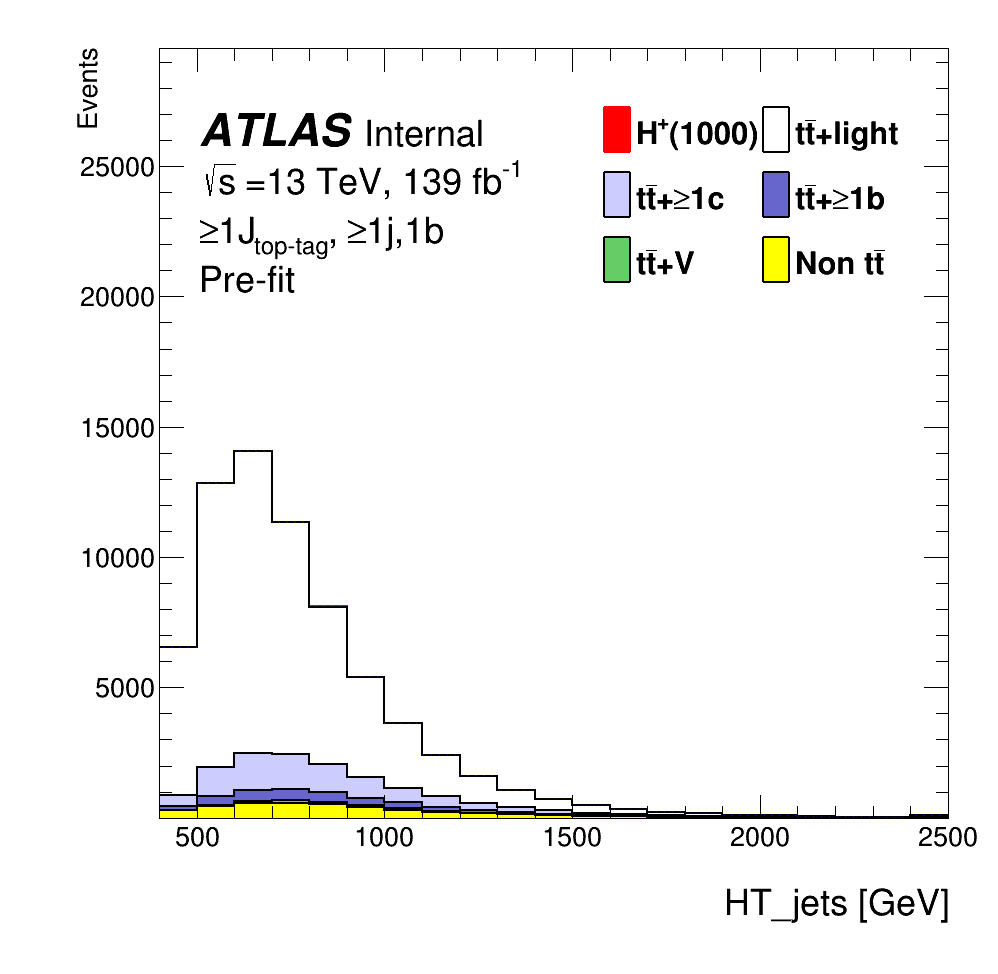
\includegraphics[keepaspectratio,scale=0.2]{images/AnalysisStrategy/HT_jets_CR_MVA.png}
    \label{fig:PieChart_SR1}
  }
  \caption{Background composition in the CR is shown in the pie chart (a) and the $H_{\text{T}}^{\text{jets}}$ distributions (b).}
  \label{fig:BkgComposition_SR2}
\end{figure}

The expected number of signal and background events in the SR and CR are shown in Table \ref{tab:PrefitYields}. For the predicted number of $H^{+}$ signal events with the 1000 and 3000 GeV mass hypothesis, the cross-section of ${\sigma}(pp{\rightarrow}tbH^{+}){\times}Br(H^{+}{\rightarrow}tb)=0.046$ pb is assumed. This corresponds to the upper limit at $M_{H^{+}}=1000$ GeV obtained from the resolved analysis \cite{HDBS-2021-02}. As discussed later in Section \ref{subsec:BlindStrategy}, we use the signal ${\sigma}{\times}Br$ to define the blinded regions. Table \ref{tab:CutflowForSignals} shows the cut flow for each signal sample.

\begin{table}[H]
  \centering
  \begin{tabular*}{120mm}{@{\extracolsep{\fill}}cll}
    \hline\hline
                            & \multicolumn{1}{c}{SR} & \multicolumn{1}{c}{CR}\\
    \hline
    $t\bar{t}+\text{light}$ & $1990\pm  95$           & $ 54008\pm 2667$ \\
    $t\bar{t}+\geq1c$       & $1063\pm 925$           & $  8011\pm 1450$ \\
    $t\bar{t}+\geq1b$       & $1853\pm 931$           & $  2793\pm 1402$ \\
    $t\bar{t}+W$            & $  38\pm   6$           & $   312\pm   41$ \\
    $t\bar{t}+Z$            & $  67\pm  11$           & $   294\pm   38$ \\
    $Wt$ channel            & $ 184\pm 107$           & $  1995\pm  742$ \\
    $t$ channel             & $  37\pm  27$           & $   172\pm   56$ \\
    Other top sources       & $   8\pm   1$           & $    34\pm    5$ \\
    $VV$, $V$+jets          & $ 152\pm  55$           & $  1529\pm  530$ \\
    $t\bar{t}H$             & $ 103\pm   4$           & $   176\pm    5$ \\
    \hline
    Total                   & $5497\pm 270$           & $ 69324\pm 3338$ \\
    \hline
    $H^{+}$ 1000 GeV        & $  56\pm  5$           & $     56\pm   10$ \\
    $H^{+}$ 3000 GeV        & $  72\pm 17$           & $     96\pm   23$ \\
    \hline\hline
  \end{tabular*}
  \caption{Number of expected events in each analysis region. The quoted uncertainties include both statistical and systematic uncertainties before fitting.}
  \label{tab:PrefitYields}
\end{table}

\begin{table}[H]
    \subfloat[] {
    \scalebox{0.70}{
    \begin{tabular*}{250mm}{@{\extracolsep{\fill}}c|cccccccccccccc}
        \hline\hline
        Mass &                        & Gen    & Reco   & TrigDec & 1$\ell$ & TrigMatch & $\geq{1J}$ & $\geq1j$ & $\geq1b^{85}$ & $\geq1J_{\text{non el}}$ & $\geq1J_{\text{top-tag}}$ & $\geq1j_{\text{add}}$ & $\geq1b^{70}_{\text{add}}$ & $\geq2b^{70}_{\text{add}}$\\
         %Mass & Cut1 & Cut2 & Cut3 & Cut4 & CUt5 & Cut6 & Cut7 & Cut8 & Cut9 & Cut10 & Cut11 & Cut12 & Cut13\\
        \hline
        1000 & $\text{N}_{\text{MC}}$ & 998000 & 541248 & 529780  & 342999  & 337300    & 256596     & 256595   & 254364        & 225152                   & 38298                     & 38259                 & 32751       
                                    & 15801\\
             & Cut eff.               & -      & 0.542  & 0.979   & 0.647   & 0.983     & 0.761      & 1.000    & 0.991         & 0.885                    & 0.170                     & 0.999                 & 0.856       
                                    & 0.482\\
        \hline
        1200 & $\text{N}_{\text{MC}}$ & 985000 & 544241 & 534601  & 335452  & 329187    & 269093     & 269093   & 266707        & 237410                   & 48012                     & 47968                 & 40768       
                                    & 19536\\
             & Cut eff.               & -      & 0.553  & 0.982   & 0.627   & 0.981     & 0.817      & 1.000    & 0.991         & 0.890                    & 0.202                     & 0.999                 & 0.850       
                                    & 0.479\\
        \hline
        1400 & $\text{N}_{\text{MC}}$ & 999000 & 560829 & 551672  & 335009  & 328190    & 280389     & 280389   & 277776        & 249152                   & 54672                     & 54626                 & 45817       
                                    & 21893\\
             & Cut eff.               & -      & 0.561  & 0.984   & 0.607   & 0.980     & 0.854      & 1.000    & 0.991         & 0.897                    & 0.219                     & 0.999                 & 0.839       
                                    & 0.478\\ 
        \hline
        1600 & $\text{N}_{\text{MC}}$ & 997000 & 565351 & 556595  & 328781  & 321427    & 282873     & 282873   & 280064        & 253245                   & 58398                     & 58374                 & 48659       
                                    & 23140\\
             & Cut eff.               & -      & 0.567  & 0.985   & 0.591   & 0.978     & 0.880      & 1.000    & 0.990         & 0.904                    & 0.231                     & 1.000                 & 0.834       
                                    & 0.476\\
        \hline
        1800 & $\text{N}_{\text{MC}}$ & 978000 & 559240 & 550740  & 315454  & 307841    & 277151     & 277151   & 273951        & 250241                   & 59500                     & 59468                 & 49081       
                                    & 22671\\
             & Cut eff.               & -      & 0.572  & 0.985   & 0.573   & 0.976     & 0.900      & 1.000    & 0.988         & 0.913                    & 0.238                     & 0.999                 & 0.825       
                                    & 0.462\\
        \hline
        2000 & $\text{N}_{\text{MC}}$ & 996000 & 570655 & 562595  & 312270  & 304274    & 278522     & 278522   & 274935        & 253344                   & 62084                     & 62056                 & 50375       
                                    & 23076\\
             & Cut eff.               & -      & 0.573  & 0.986   & 0.555   & 0.974     & 0.915      & 1.000    & 0.987         & 0.921                    & 0.245                     & 1.000                 & 0.812       
                                    & 0.458\\
        \hline
        2500 & $\text{N}_{\text{MC}}$ & 999000 & 574372 & 566804  & 294566  & 286030    & 268297     & 268297   & 263948        & 248193                   & 64809                     & 64780                 & 51192                                     & 22231\\
             & Cut eff.               & -      & 0.575  & 0.987   & 0.520   & 0.971     & 0.938      & 1.000    & 0.984         & 0.940                    & 0.261                     & 1.000                 & 0.790                                & 0.434\\
        \hline
        3000 & $\text{N}_{\text{MC}}$ & 999000 & 570796 & 563605  & 277515  & 268587    & 255972     & 255972   & 250995        & 239429                   & 66834                     & 66826                 & 51600                                     & 21345\\
             & Cut eff.               & -      & 0.571  & 0.987   & 0.492   & 0.968     & 0.953      & 1.000    & 0.981         & 0.954                    & 0.279                     & 1.000                 & 0.772         
                                    & 0.413\\         
        \hline\hline
    \end{tabular*}
    \label{tab:CutflowForHp}
    }
    }\par
\end{table}

\begin{table}[H]
    \subfloat[]{
    \scalebox{0.70}{
    \begin{tabular*}{250mm}{@{\extracolsep{\fill}}c|cccccccccccccc}
        \hline\hline
        Mass &                        & Gen    & Reco   & TrigDec & 1$\ell$ & TrigMatch & $\geq{1J}$ & $\geq1j$ & $\geq1b^{85}$ & $\geq1J_{\text{non el}}$ & $\geq1J_{\text{top-tag}}$ & $\geq1j_{\text{add}}$ & $\geq1b^{70}_{\text{add}}$ & $\geq2b^{70}_{\text{add}}$\\
        \hline
        1000 & $\text{N}_{\text{MC}}$ & 498000 & 248196 & 241900  & 151833  & 148932    & 118640     & 118640   & 117932        & 107739                   & 18538                     & 18534                 & 16264                                    & 8623\\
             & Cut eff.               & -      & 0.498  & 0.975   & 0.628   & 0.981     & 0.797      & 1.000    & 0.994         & 0.914                    & 0.172                     & 1.000                 & 0.878                               & 0.530\\
        \hline
        1200 & $\text{N}_{\text{MC}}$ & 497000 & 254395 & 248661  & 152134  & 148969    & 125935     & 125935   & 125170        & 114663                   & 22658                     & 22653                 & 19664         
                                   & 10291\\
             & Cut eff.               & -      & 0.512  & 0.977   & 0.612   & 0.979     & 0.845      & 1.000    & 0.994         & 0.916                    & 0.198                     & 1.000                 & 0.868                               & 0.523\\
        \hline
        1400 & $\text{N}_{\text{MC}}$ & 499000 & 260545 & 255004  & 151933  & 148562    & 130183     & 130183   & 129327        & 118716                   & 24673                     & 24667                 & 21203                                    & 11079\\
             & Cut eff.               & -      & 0.522  & 0.979   & 0.596   & 0.978     & 0.876      & 1.000    & 0.993         & 0.918                    & 0.208                     & 1.000                 & 0.860                               & 0.523\\
        \hline
        1600 & $\text{N}_{\text{MC}}$ & 497000 & 263865 & 258714  & 150482  & 146957    & 131867     & 131867   & 130959        & 121196                   & 26420                     & 26412                 & 22631                                    & 11616\\
             & Cut eff.               & -      & 0.531  & 0.980   & 0.582   & 0.977     & 0.897      & 1.000    & 0.993         & 0.925                    & 0.218                     & 1.000                 & 0.857                               & 0.513\\
        \hline
        1800 & $\text{N}_{\text{MC}}$ & 490000 & 263070 & 258072  & 145536  & 141752    & 129382     & 129382   & 128408        & 119539                   & 27016                     & 27014                 & 22925                                    & 11728\\
             & Cut eff.               & -      & 0.537  & 0.981   & 0.564   & 0.974     & 0.913      & 1.000    & 0.992         & 0.931                    & 0.226                     & 1.000                 & 0.849                               & 0.512\\
        \hline
        2000 & $\text{N}_{\text{MC}}$ & 500000 & 269918 & 265056  & 145830  & 141828    & 131486     & 131486   & 130372        & 122004                   & 28059                     & 28053                 & 23583                                    & 11914\\
             & Cut eff.               & -      & 0.540  & 0.982   & 0.550   & 0.973     & 0.927      & 1.000    & 0.992         & 0.936                    & 0.230                     & 1.000                 & 0.841         
                                   & 0.505\\
        \hline
        2500 & $\text{N}_{\text{MC}}$ & 497000 & 271566 & 267051  & 137291  & 133192    & 125774     & 125774   & 124454        & 117931                   & 29003                     & 28999                 & 23868                                    & 11596\\
             & Cut eff.               & -      & 0.546  & 0.983   & 0.514   & 0.970     & 0.944      & 1.000    & 0.990         & 0.948                    & 0.246                     & 1.000                 & 0.823                               & 0.486\\
        \hline
        3000 & $\text{N}_{\text{MC}}$ & 489000 & 267310 & 262927  & 126289  & 121989    & 116513     & 116513   & 115007        & 109992                   & 28753                     & 28750                 & 23174                                    & 10622\\
             & Cut eff.               & -      & 0.547  & 0.984   & 0.480   & 0.966     & 0.955      & 1.000    & 0.987         & 0.956                    & 0.261                     & 1.000                 & 0.806         
                                   & 0.458\\ 
        \hline\hline
    \end{tabular*}
    \label{tab:CutflowForWpLH}
    }
    }\par

    \subfloat[]{
    \scalebox{0.70}{
    \begin{tabular*}{250mm}{@{\extracolsep{\fill}}c|cccccccccccccc}
        \hline\hline
        Mass &                        & Gen    & Reco   & TrigDec & 1$\ell$ & TrigMatch & $\geq{1J}$ & $\geq1j$ & $\geq1b^{85}$ & $\geq1J_{\text{non el}}$ & $\geq1J_{\text{top-tag}}$ & $\geq1j_{\text{add}}$ & $\geq1b^{70}_{\text{add}}$ & $\geq2b^{70}_{\text{add}}$\\
        \hline
        1000 & $\text{N}_{\text{MC}}$ & 499000 & 294866 & 290492  & 186576  & 183583    & 147606     & 147606   & 146329        & 131251                   & 24304                     & 24293                 & 21011                                    & 10895\\
             & Cut eff.               & -      & 0.591  & 0.985   & 0.642   & 0.984     & 0.804      & 1.000    & 0.991         & 0.897                    & 0.185                     & 1.000                 & 0.865                               & 0.519\\
        \hline
        1200 & $\text{N}_{\text{MC}}$ & 500000 & 300323 & 296365  & 185318  & 181937    & 154413     & 154413   & 153000        & 138404                   & 29012                     & 28997                 & 24801                                    & 12811\\
             & Cut eff.               & -      & 0.601  & 0.987   & 0.625   & 0.982     & 0.849      & 1.000    & 0.991         & 0.905                    & 0.210                     & 1.000                 & 0.855         
                                   & 0.517\\
        \hline
        1400 & $\text{N}_{\text{MC}}$ & 500000 & 303573 & 299866  & 181675  & 178152    & 156905     & 156905   & 155480        & 141630                   & 32480                     & 32470                 & 27571                                    & 13870\\
             & Cut eff.               & -      & 0.607  & 0.988   & 0.606   & 0.981     & 0.881      & 1.000    & 0.991         & 0.911                    & 0.229                     & 1.000                 & 0.849         
                                   & 0.503\\
        \hline
        1600 & $\text{N}_{\text{MC}}$ & 498000 & 304438 & 300981  & 177434  & 173574    & 156104     & 156104   & 154405        & 141953                   & 34356                     & 34336                 & 28999                                    & 14487\\
             & Cut eff.               & -      & 0.611  & 0.989   & 0.590   & 0.978     & 0.899      & 1.000    & 0.989         & 0.919                    & 0.242                     & 0.999                 & 0.845                               & 0.500\\
        \hline
        1800 & $\text{N}_{\text{MC}}$ & 488000 & 299636 & 296508  & 170489  & 166656    & 152480     & 152480   & 150711        & 139586                   & 34423                     & 34413                 & 28710                                    & 14220\\
             & Cut eff.               & -      & 0.614  & 0.990   & 0.575   & 0.978     & 0.915      & 1.000    & 0.988         & 0.926                    & 0.247                     & 1.000                 & 0.834                               & 0.495\\
        \hline
        2000 & $\text{N}_{\text{MC}}$ & 488000 & 300376 & 297075  & 166140  & 162131    & 150247     & 150247   & 148297        & 138313                   & 35279                     & 35265                 & 29166                                    & 14182\\
             & Cut eff.               & -      & 0.616  & 0.989   & 0.559   & 0.976     & 0.927      & 1.000    & 0.987         & 0.933                    & 0.255                     & 1.000                 & 0.827                               & 0.486\\
        \hline
        2500 & $\text{N}_{\text{MC}}$ & 498000 & 305572 & 302770  & 159971  & 155580    & 146930     & 146930   & 144597        & 136696                   & 36850                     & 36841                 & 29578                                    & 13558\\
             & Cut eff.               & -      & 0.614  & 0.991   & 0.528   & 0.973     & 0.944      & 1.000    & 0.984         & 0.945                    & 0.270                     & 1.000                 & 0.802         
                                   & 0.458\\
        \hline
        3000 & $\text{N}_{\text{MC}}$ & 499000 & 304217 & 301493  & 152213  & 147658    & 140988     & 140988   & 138344        & 132052                   & 37948                     & 37944                 & 29674                                    & 13047\\
             & Cut eff.               & -      & 0.610  & 0.991   & 0.504   & 0.970     & 0.955      & 1.000    & 0.981         & 0.955                    & 0.287                     & 1.000                 & 0.782                               & 0.440\\
        \hline\hline
    \end{tabular*}
    \label{tab:CutflowForWpRH}
    }
    }
    \caption{Cut flow for the $H^{+}$ (a), $W'_{\text{LH}}$ (b), and $W'_{\text{RH}}$ (c) signal: for each sample the corresponding mass, the number of generated events (Gen), the number of reconstructed events (Reco), the number of events that pass lepton triggers (TrigDec), the number of events that have an electron or muon with $p_{\text{T}}$ larger than 27 GeV ($1\ell$), the number of events that the lepton matches to the one detected with the trigger (TrigMatch), the number of events that have at least one large-R jets with $p_{\text{T}}$ larger than 200 GeV ($\geq1J$), the number of events that have at least one small-R jets with $p_{\text{T}}$ larger than 25 GeV ($\geq1j$), the number of events that have at least one $b$-tagged jets at the 85\% efficiency working point ($\geq1b^{85}$), the number of events that have at least one large-R jets with ${\Delta}R$ to the electron smaller than 1.0 ($\geq1J_{\text{non el}}$), the number of events that have at least one top-tagged large-R jets with contained top-tagger at the 80\% efficiency working point ($\geq1J_{\text{top-tag}}$), the number of events that have at least additional small-R jets with ${\Delta}R$ to the leading top-tagged large-R jet larger than 1.0 ($\geq1j_{\text{add}}$), the number of events that have at least one or two $b$-tagged additional small-R jets at the 70\% efficiency working point ($\geq1b^{70}$, $\geq2b^{70}$ ) are shown in the top rows ($\text{N}_{\text{MC}}$). Each cut efficiency is also shown in the bottom rows (Cut eff.).}
    \label{tab:CutflowForSignals}
\end{table}


\subsubsection{Multivariable analysis using BDT}
\label{subsubsec:MVA}

In this search, the most important background is $t\bar{t}+\text{jets}$ as discussed in Section \ref{subsec:AnaStrategyUnder3TeV}. To enhance the separation between signal and background, multivariable analysis is performed using Boosted Decision Trees (BDT) technique of TMVA \cite{TMVA}. Obtained BDT score distribution is used in the profile likelihood fit as a final discriminant (Section \ref{sec:ProfileLikelohoodFit}).

\begin{description}
    \item{\textbf{Signal and background definition in BDT training}}\mbox{}\\
    To classify signal ($H^{+}$ and $W'$) and $t\bar{t}+\text{jets}$ background events, BDTs are trained using the simulated $H^{+}$ signal and $t\bar{t}+\text{jets}$ background samples. This analysis under 3 TeV mass points considers eight different mass hypotheses, and the training is performed on each mass hypothesis. On the other hand, the $t\bar{t}+\text{jets}$ background samples are common in each training. Since kinematics of $H^+$ signals become harder in higher mass hypotheses, the BDTs trained using the higher $H^{+}$ mass samples typically have greater separation power. These signal events and background events used in training are required to pass either SR criteria. These BDTs optimized using $H^{+}$ signal samples can be also used in $W' \rightarrow tb$ analysis because the difference between a $H^{+}$ and $W'$ is only their spin and the kinematic characteristics of $W' \rightarrow tb$ events are similar to the ones of $H^{+} \rightarrow tb$ events. This validation is done in the section below. BDTs are also trained using 4 and 5 TeV mass point samples. These BDT outputs are only used for the study in Section \ref{subsec:ReweightingTechnique}.

    \item{\textbf{BDT training settings}}\mbox{}\\
    To fully use the simulation samples' statistics, we adopt the 4-fold cross-validation method in the BDT training (Figure \ref{fig:CrossValidationScheme}). Each simulation sample is divided into four sub-datasets (Fold1, Fold2, Fold3, and Fold4). For each MC event, a random number is generated with the MC event number as a seed, and the event is categorized into one of the sub-datasets according to the generated number. Two of the four sub-datasets are labelled "TRAIN," which are used for BDT training. One of the other sub-datasets is labelled "VALID" and is used to optimize the BDT performance. The last sample, "TEST", is used to construct a fit template. Four combinations of sub-dataset usage (Split1 to Split4 in Figure \ref{fig:CrossValidationScheme}) are tried, and we obtain four statistically-independent BDTs and fit templates. They are combined into one fit template used in the profile likelihood fit (Section.\ref{sec:ProfileLikelohoodFit}).
    
    \begin{figure}[H]
        \centering
        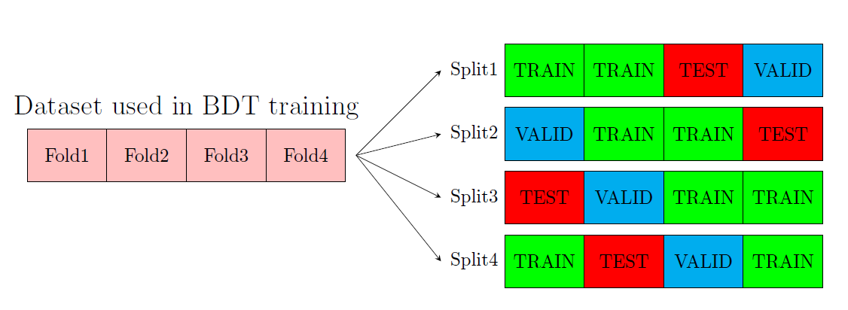
\includegraphics[keepaspectratio,scale=0.65]{images/AnalysisStrategy/CrossValidationScheme.png}
        \caption{Scheme of 4-fold cross-validation of BDT in this analysis.}
        \label{fig:CrossValidationScheme}
    \end{figure}
    
    Hyperparameters for the BDTs are summarized in Table. \ref{tab:Hyperparameters}. Those hyperparameters are chosen to obtain the best sensitivity.

    \begin{table}[H]
      \centering
      \begin{tabular*}{75mm}{@{\extracolsep{\fill}}ll}
        \hline
        \multicolumn{1}{c}{Configuration} & \multicolumn{1}{c}{}\\
        \hline\hline
        \multicolumn{1}{l}{Algorithm}     & \multicolumn{1}{c}{Gradient boosting}\\
        \hline
        $Hyperparameters$ & \\
        \multicolumn{1}{l}{NTrees}       & \multicolumn{1}{c}{100}\\
        \multicolumn{1}{l}{MinNodeSize}  & \multicolumn{1}{c}{2.5}\\
        \multicolumn{1}{l}{MaxDepth}     & \multicolumn{1}{c}{3}\\
        \multicolumn{1}{l}{nCuts}        & \multicolumn{1}{c}{20}\\
        \hline
      \end{tabular*}
      \caption{List of hyperparameters used in the training of a BDT}
      \label{tab:Hyperparameters}
    \end{table}

    \item{\textbf{Input variables in BDT}}\mbox{}\\
    \label{item:BDTInputVars}
    Jets originating from a $H^{+}$ ($W'$) decay have higher $p_\text{T}$ comparing with $t\bar{t}+\text{jets}$ events due to its heavy mass. Additionally, angular and kinematics correlation among jets are different between $H^{+}$ ($W'$) and $t\bar{t}+\text{jets}$ events because these bosons create a resonance. The BDT is trained to exploit these kinematic characteristics fully. The variables used in BDT training are summarized in Table \ref{tab:BDTInputVariables}. Any variables for missing $E_{T}$ are not used in BDT training. In Figure \ref{fig:SOVERB_Hp3000_Contained80_DL1r_70}, each distribution in the $H^{+}$ sample with a mass of 3000~GeV is compared with the $t\bar{t}+\text{jets}$ background. Table \ref{tab:RankingOfBDTInputVariables_Hp3000} shows the ranking of these variables.

    \begin{table}[H]
      \centering
      \begin{tabular*}{150mm}{@{\extracolsep{\fill}}ll}
        \hline
        \multicolumn{1}{c}{Symbol} & \multicolumn{1}{c}{Description}\\
        \hline\hline
        HT\_jets                                   & Scalar sum of the transverse energy of all jets\\
        LeadingJet\_pt                             & Leading jet $p_\text{T}$\\
        Mjjj\_MaxPt                                & Invariant mass of the jet triplet with maximum $p_\text{T}$\\
        Mbb\_MaxPt                                 & Invariant mass of the b-jet pair with maximum $p_\text{T}$\\
        Muu\_MindR                                 & Invariant mass of the untagged jet-pair with minimum $\Delta{R}$\\
        dRlepbb\_MindR                             & $\Delta{R}$ between the lepton and the pair of $b$-jets with smallest $\Delta{R}$\\
        dRbb\_avg                                  & Average $\Delta{R}$ between all $b$-jet pairs in the event\\
        Centrality\_all                            & Centrality calculated using all jets and leptons\\
        H1\_all                                    & Second Fox-Wolfram moment calculated using all jets and lepton\\
        LeadingTop\_pt                             & Leading top-tagged jet $p_\text{T}$\\
        LeadingTop\_m                              & Invariant mass of leading top-tagged jet \\
        Pt\_tb                                     & $p_\text{T}$ of the pair of leading top-tagged jet and leading $b$-jet\\
        M\_tb                                      & Invariant mass of the pair of leading top-tagged jet and leading $b$-jet\\
        PtAsymm\_tb                                & $p_\text{T}$ asymmetry between leading top-tagged jet and leading $b$-jet\\
        \hline
      \end{tabular*}
      \caption{List of variables included in the training of the BDT}
      \label{tab:BDTInputVariables}
    \end{table}

    %--- Ranking @H+(3000)
    \begin{table}[H]
      \centering
      \begin{tabular*}{160mm}{@{\extracolsep{\fill}}lllllll}
        \hline\hline
        \multirow{2}{*}{Ranking} & \multirow{2}{*}{Variable} & \multicolumn{5}{c}{Importance}\\
                                 &                           & Fold1 & Fold2 & Fold3 & Fold4 & Avg.\\
        \hline
        1  & HT\_jets        & 9.509E-02 & 1.118E-01 & 1.216E-01 & 1.073E-01 & 1.089E-01\\
        2  & Centrality\_all & 1.053E-01 & 9.995E-02 & 1.126E-01 & 1.012E-01 & 1.048E-01\\
        3  & M\_tb           & 9.192E-02 & 9.473E-02 & 8.282E-02 & 8.014E-02 & 8.740E-02\\
        4  & LeadingTop\_pt  & 8.710E-02 & 8.107E-02 & 6.472E-02 & 7.292E-02 & 7.645E-02\\
        5  & Pt\_tb          & 7.944E-02 & 7.816E-02 & 7.888E-02 & 6.795E-02 & 7.611E-02\\
        6  & LeadingJet\_pt  & 6.180E-02 & 7.860E-02 & 6.628E-02 & 7.577E-02 & 7.061E-02\\
        7  & dRlepbb\_MindR  & 6.997E-02 & 7.842E-02 & 6.968E-02 & 6.393E-02 & 7.050E-02\\
        8  & dRbb\_avg       & 6.236E-02 & 6.435E-02 & 5.331E-02 & 7.843E-02 & 6.461E-02\\
        9  & Mbb\_MaxPt      & 5.348E-02 & 6.657E-02 & 7.339E-02 & 5.552E-02 & 6.224E-02\\
        10 & PtAsymm\_tb     & 5.209E-02 & 6.526E-02 & 5.843E-02 & 6.620E-02 & 6.050E-02\\
        11 & Mjjj\_MaxPt     & 6.439E-02 & 6.248E-02 & 5.503E-02 & 5.577E-02 & 5.942E-02\\
        12 & H1\_all         & 6.316E-02 & 4.577E-02 & 4.876E-02 & 6.291E-02 & 5.515E-02\\
        13 & LeadingTop\_m   & 5.868E-02 & 3.864E-02 & 5.567E-02 & 5.748E-02 & 5.262E-02\\
        14 & Muu\_MindR      & 4.438E-02 & 3.422E-02 & 5.889E-02 & 5.439E-02 & 4.797E-02\\
        \hline\hline
      \end{tabular*}
      \caption{Importance ranking of variables used in BDT training on 3000 GeV H+ mass hypothesis. Importance values are output from TMVA.}
      \label{tab:RankingOfBDTInputVariables_Hp3000}
    \end{table}

    \begin{figure}[H]
      \subfloat[HT\_jets] {
        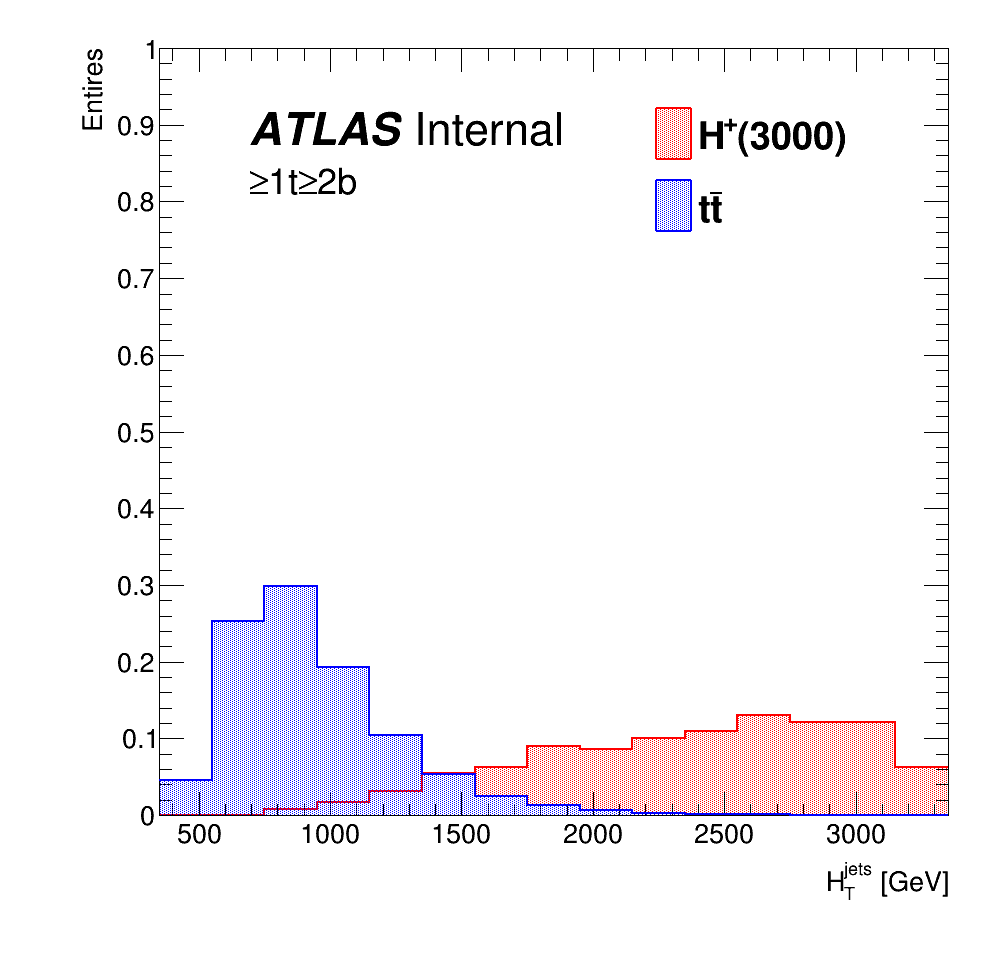
\includegraphics[width=0.25\textwidth]{images/AnalysisStrategy/SOVERB_Hp3000_Contained80_DL1r_70_HT_jets_Contained80_DL1r_70.png}
        \label{fig:SOVERB_HT_jets_Hp3000_Contained80_DL1r_70}
      }
      \subfloat[LeadingJet\_pt] {
        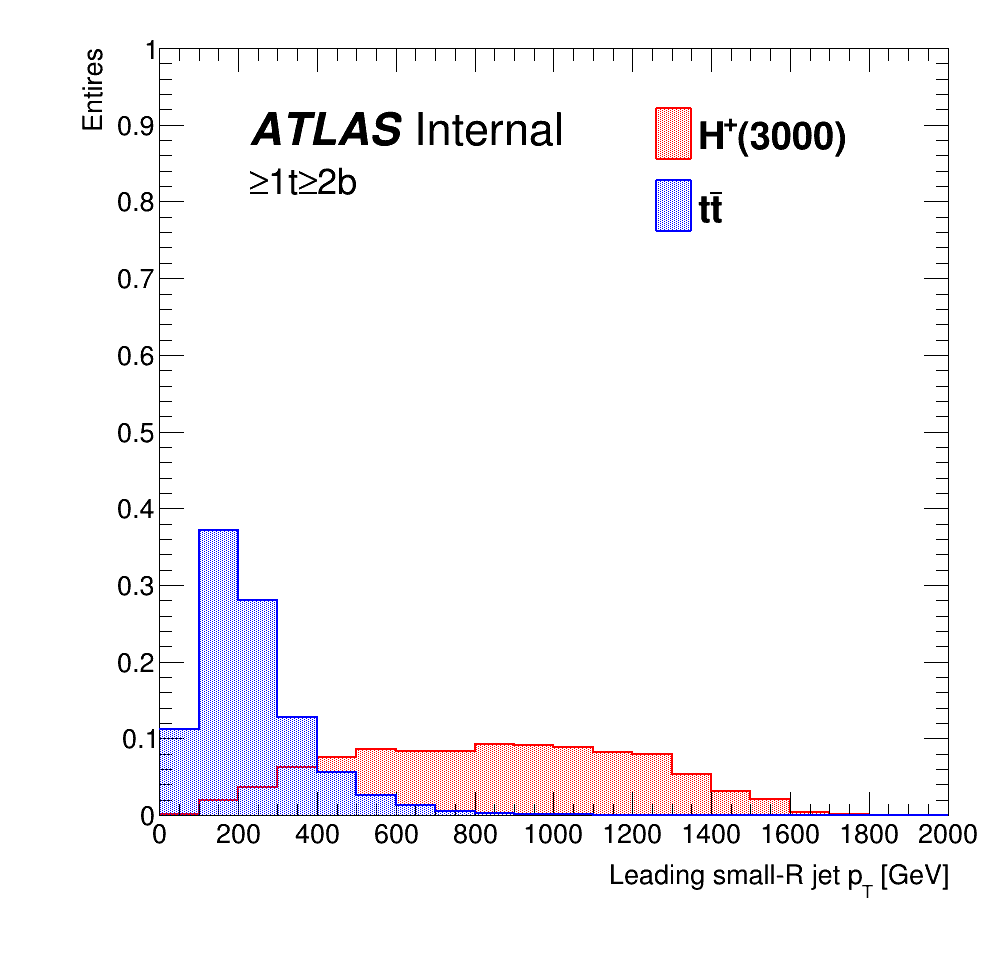
\includegraphics[width=0.25\textwidth]{images/AnalysisStrategy/SOVERB_Hp3000_Contained80_DL1r_70_leadingJet_pt_Contained80_DL1r_70.png}
        \label{fig:SOVERB_LeadingJet_pt_Hp3000_Contained80_DL1r_70}
      }
      \subfloat[Centrality\_all] {
        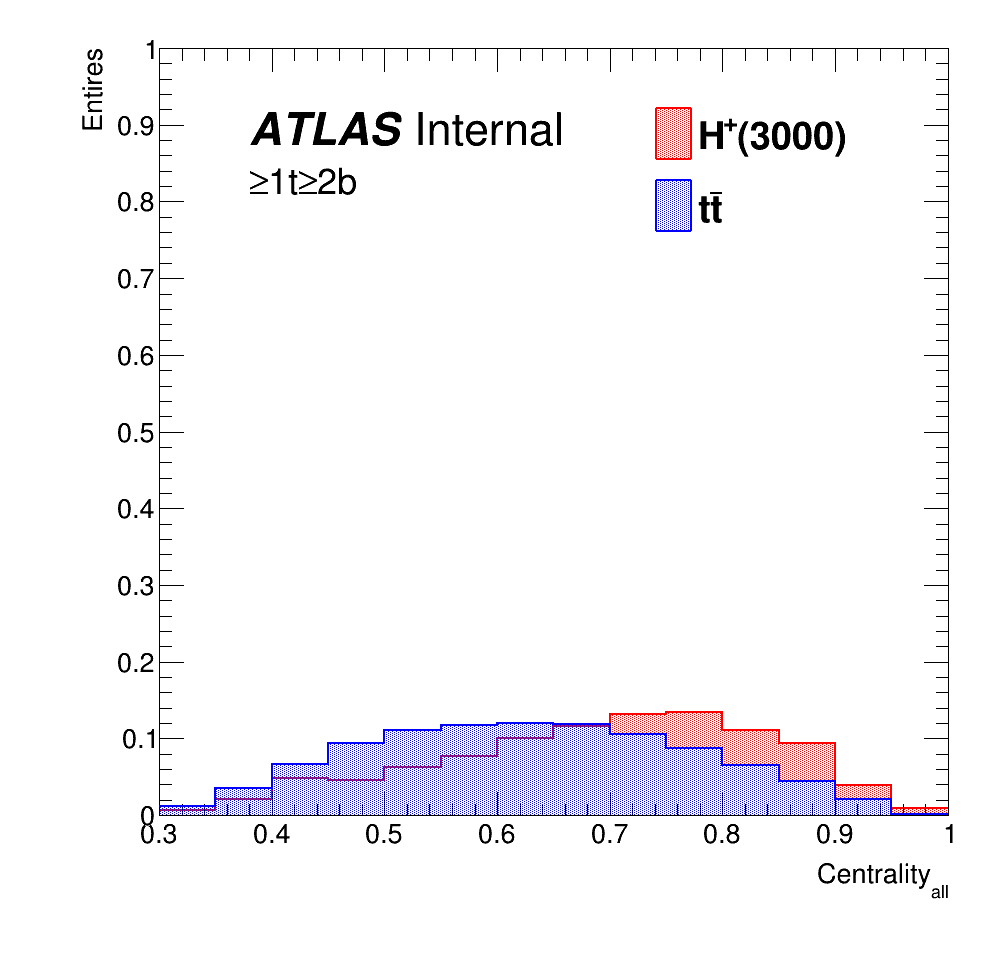
\includegraphics[width=0.25\textwidth]{images/AnalysisStrategy/SOVERB_Hp3000_Contained80_DL1r_70_Centrality_all_Contained80_DL1r_70.png}
        \label{fig:SOVERB_Centrality_all_Hp3000_Contained80_DL1r_70}
      }
      \subfloat[H1\_all] {
        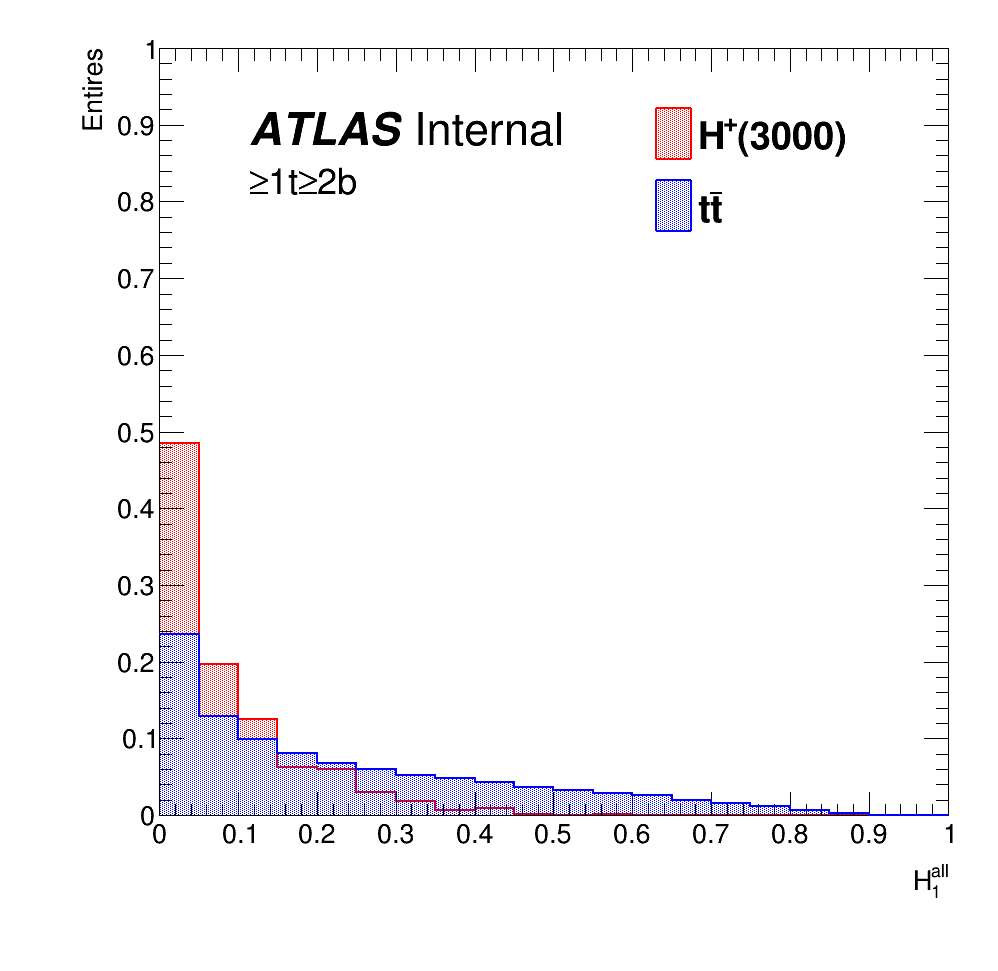
\includegraphics[width=0.25\textwidth]{images/AnalysisStrategy/SOVERB_Hp3000_Contained80_DL1r_70_H1_all_Contained80_DL1r_70.png}
        \label{fig:SOVERB_H1_all_Hp3000_Contained80_DL1r_70}
      }\\
      \subfloat[Mbb\_MaxPt] {
        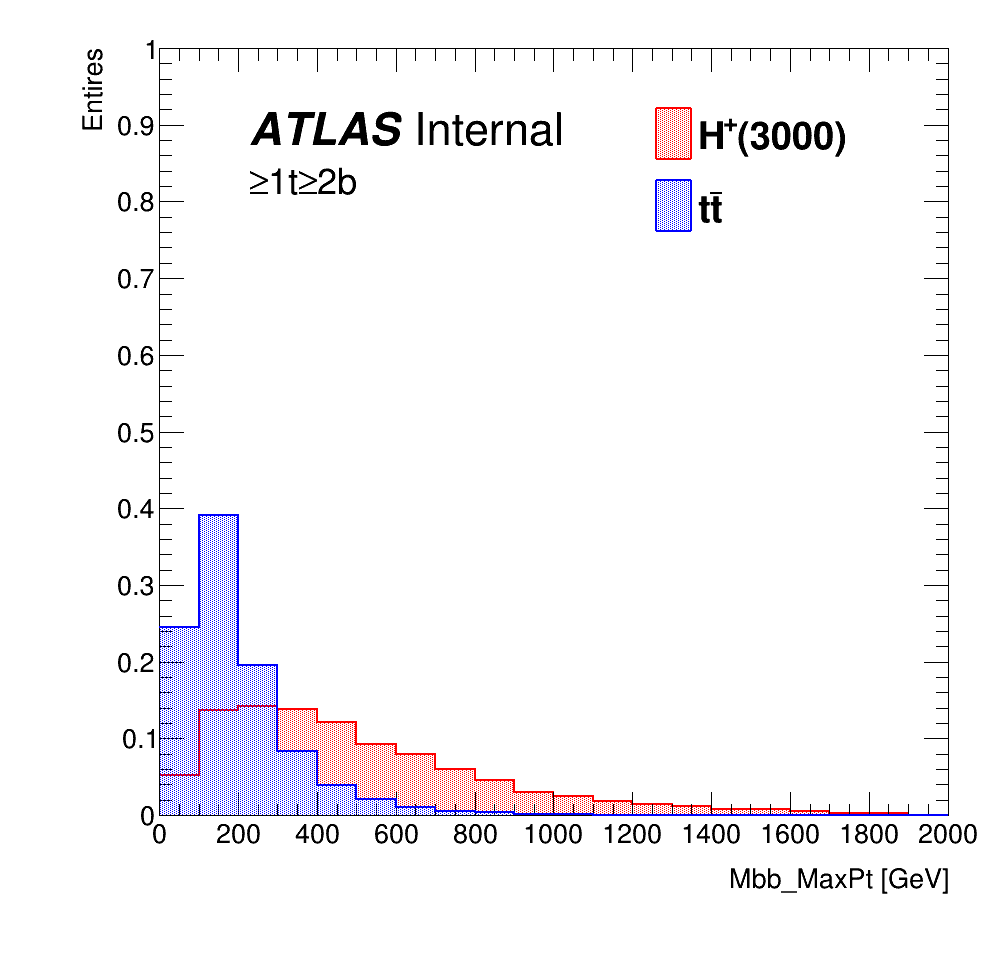
\includegraphics[width=0.25\textwidth]{images/AnalysisStrategy/SOVERB_Hp3000_Contained80_DL1r_70_Mbb_MaxPt_Contained80_DL1r_70.png}
        \label{fig:SOVERB_Mbb_MaxPt_Hp3000_Contained80_DL1r_70}
      }
      \subfloat[Mjjj\_MaxPt] {
        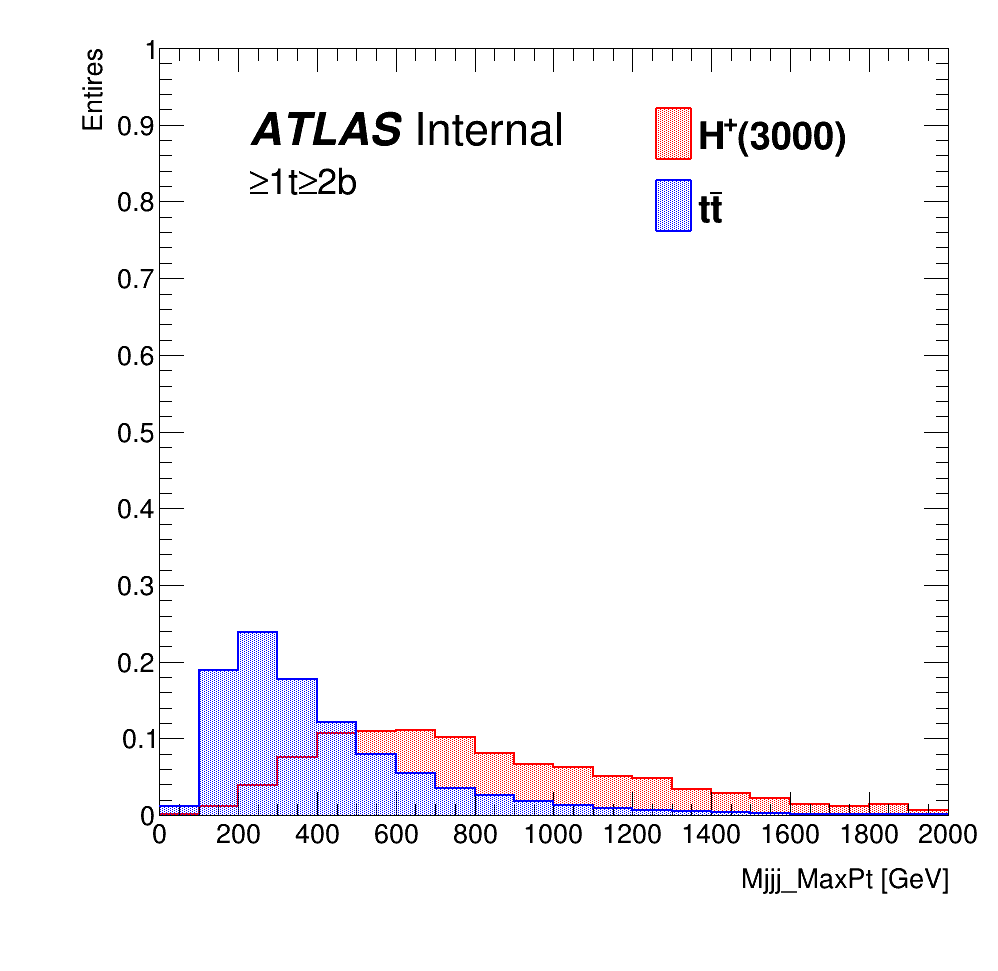
\includegraphics[width=0.25\textwidth]{images/AnalysisStrategy/SOVERB_Hp3000_Contained80_DL1r_70_Mjjj_MaxPt_Contained80_DL1r_70.png}
        \label{fig:SOVERB_Mjjj_MaxPt_Hp3000_Contained80_DL1r_70}
      }
      \subfloat[Muu\_MindR] {
        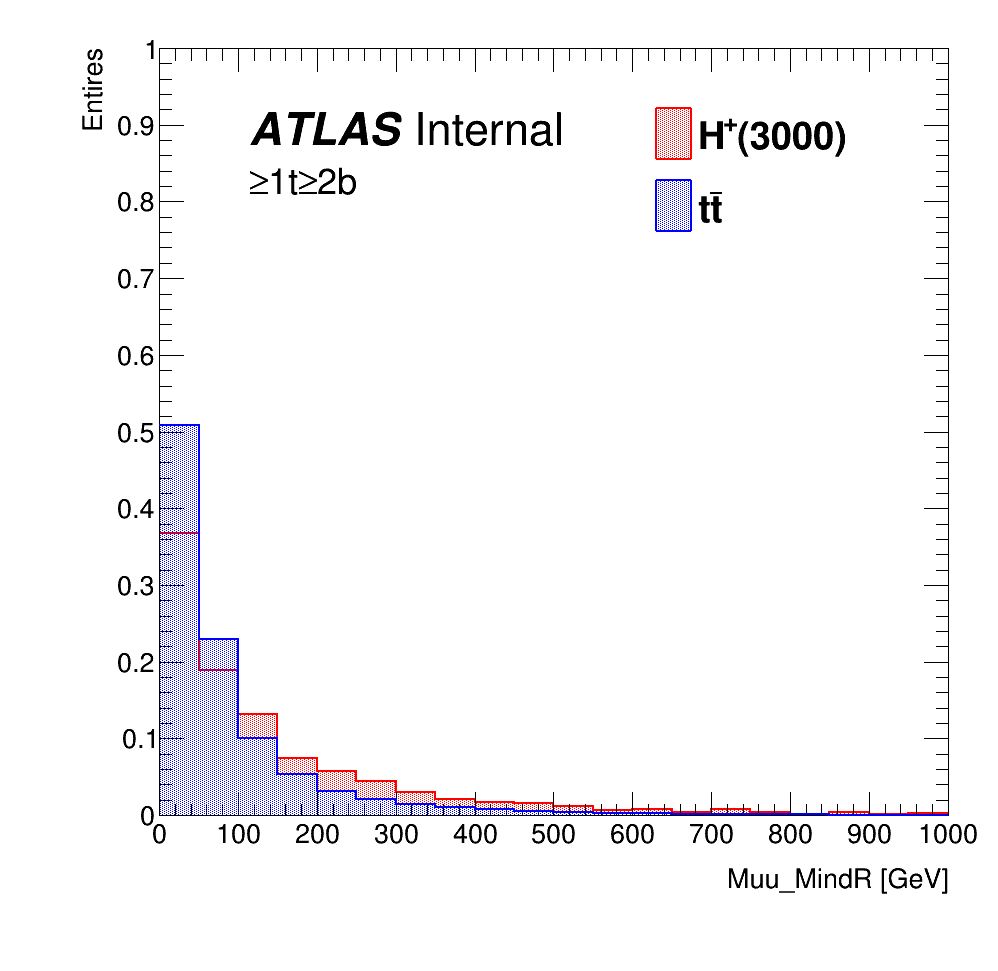
\includegraphics[width=0.25\textwidth]{images/AnalysisStrategy/SOVERB_Hp3000_Contained80_DL1r_70_Muu_MindR_Contained80_DL1r_70.png}
        \label{fig:SOVERB_Muu_MindR_Hp3000_Contained80_DL1r_70}
      }
      \subfloat[dRbb\_avg] {
        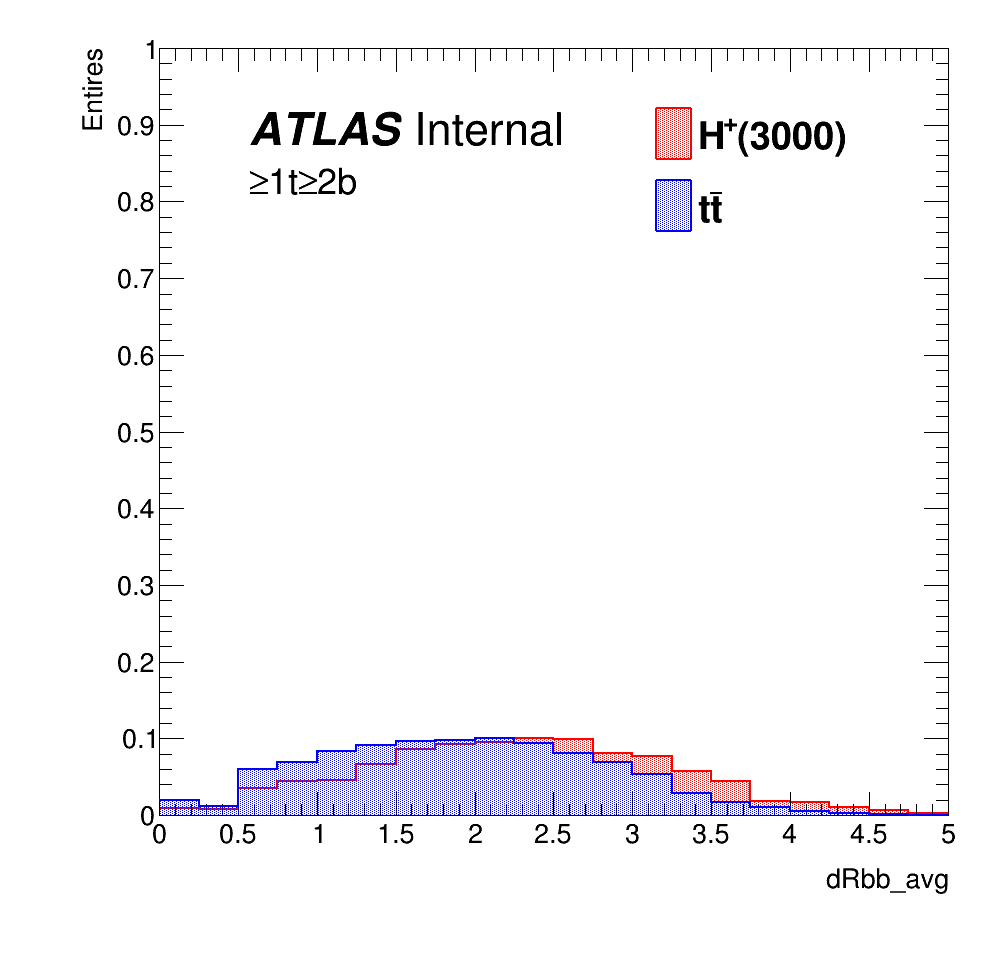
\includegraphics[width=0.25\textwidth]{images/AnalysisStrategy/SOVERB_Hp3000_Contained80_DL1r_70_dRbb_avg_Contained80_DL1r_70.png}
        \label{fig:SOVERB_dRbb_avg_Hp3000_Contained80_DL1r_70}
      }\\
      \subfloat[dRlepbb\_MindR] {
        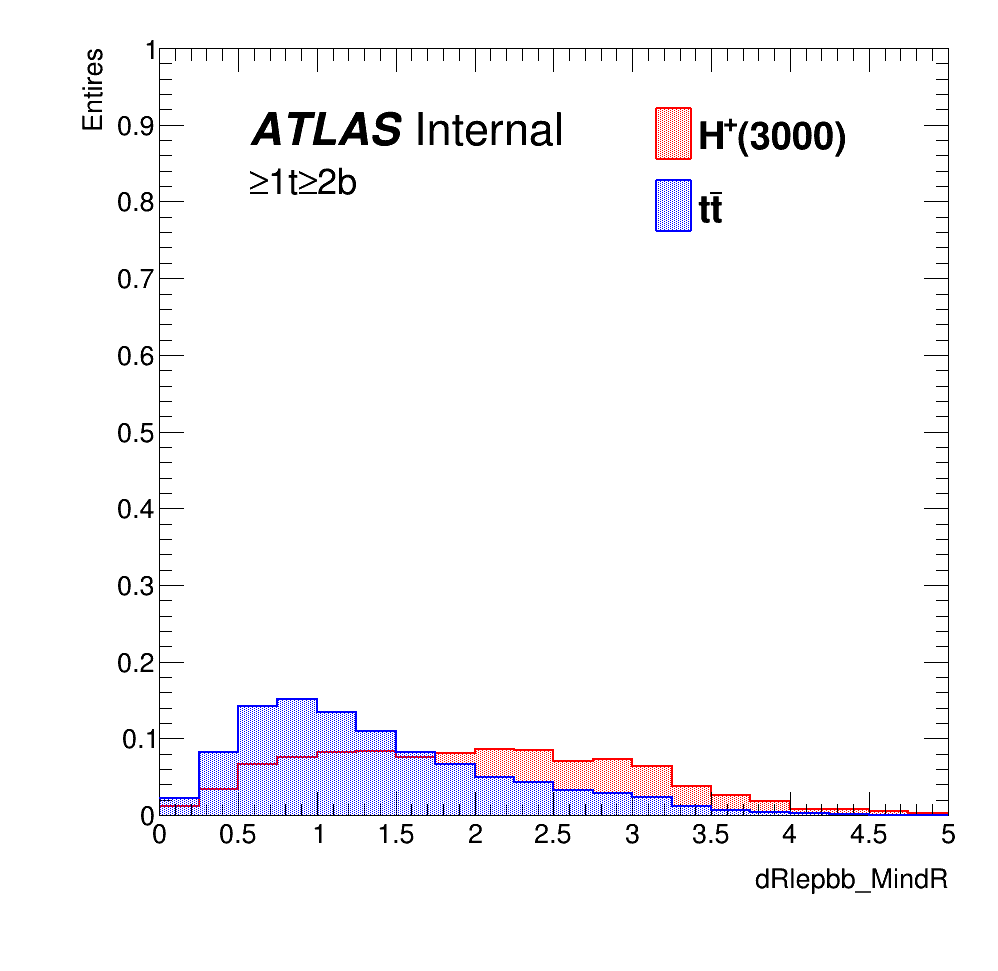
\includegraphics[width=0.25\textwidth]{images/AnalysisStrategy/SOVERB_Hp3000_Contained80_DL1r_70_dRlepbb_MindR_Contained80_DL1r_70.png}
        \label{fig:SOVERB_dRlepbb_MindR_Hp3000_Contained80_DL1r_70}
      }
      \subfloat[LeadingTop\_m] {
        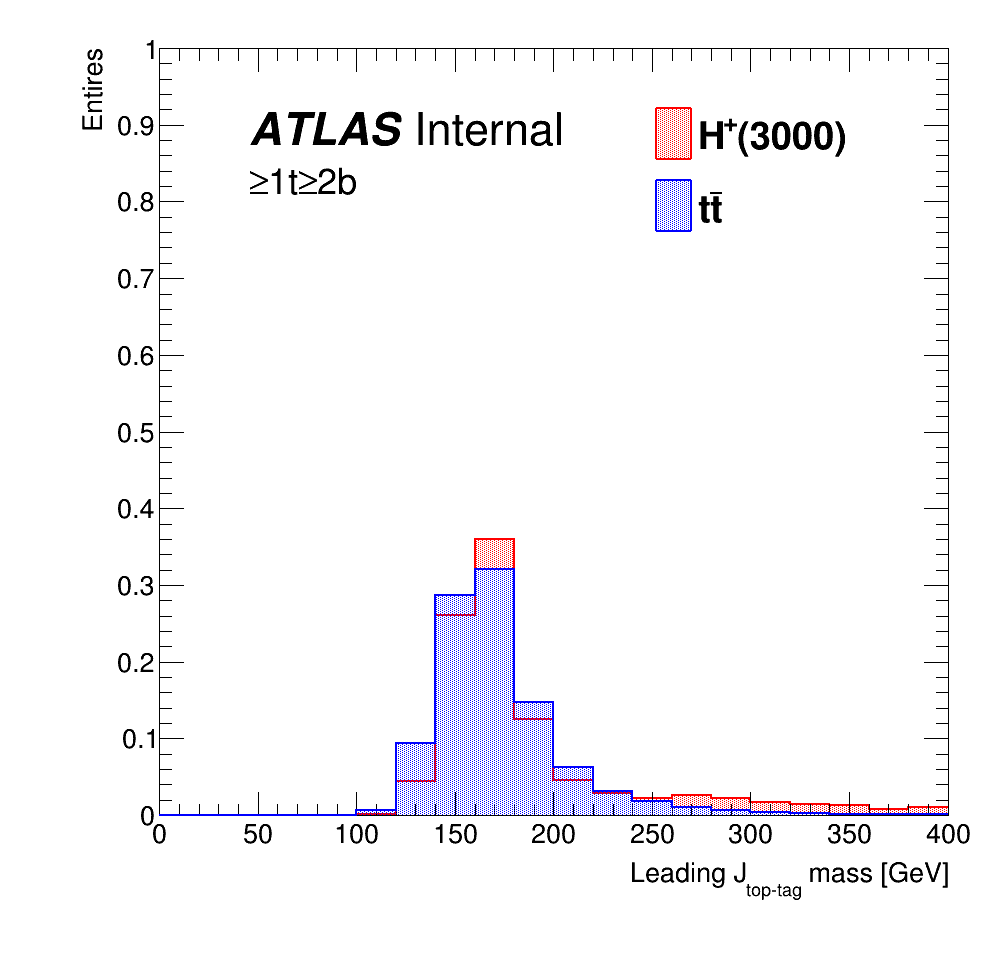
\includegraphics[width=0.25\textwidth]{images/AnalysisStrategy/SOVERB_Hp3000_Contained80_DL1r_70_leadingTop_m_Contained80_DL1r_70.png}
        \label{fig:SOVERB_leadingTop_mass_Hp3000_Contained80_DL1r_70}
      }
      \subfloat[LeadingTop\_pt] {
        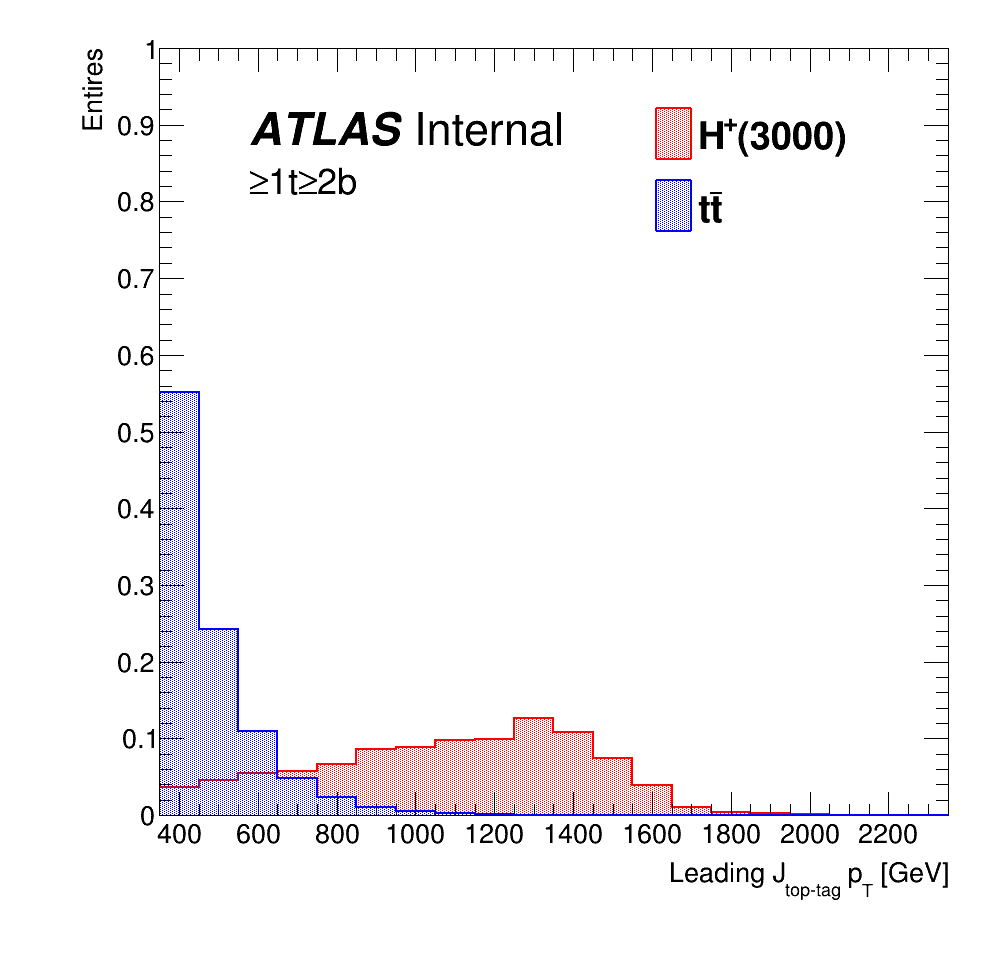
\includegraphics[width=0.25\textwidth]{images/AnalysisStrategy/SOVERB_Hp3000_Contained80_DL1r_70_leadingTop_pt_Contained80_DL1r_70.png}
        \label{fig:SOVERB_leadingTop_pt_Hp3000_Contained80_DL1r_70}
      }
      \subfloat[M\_tb] {
        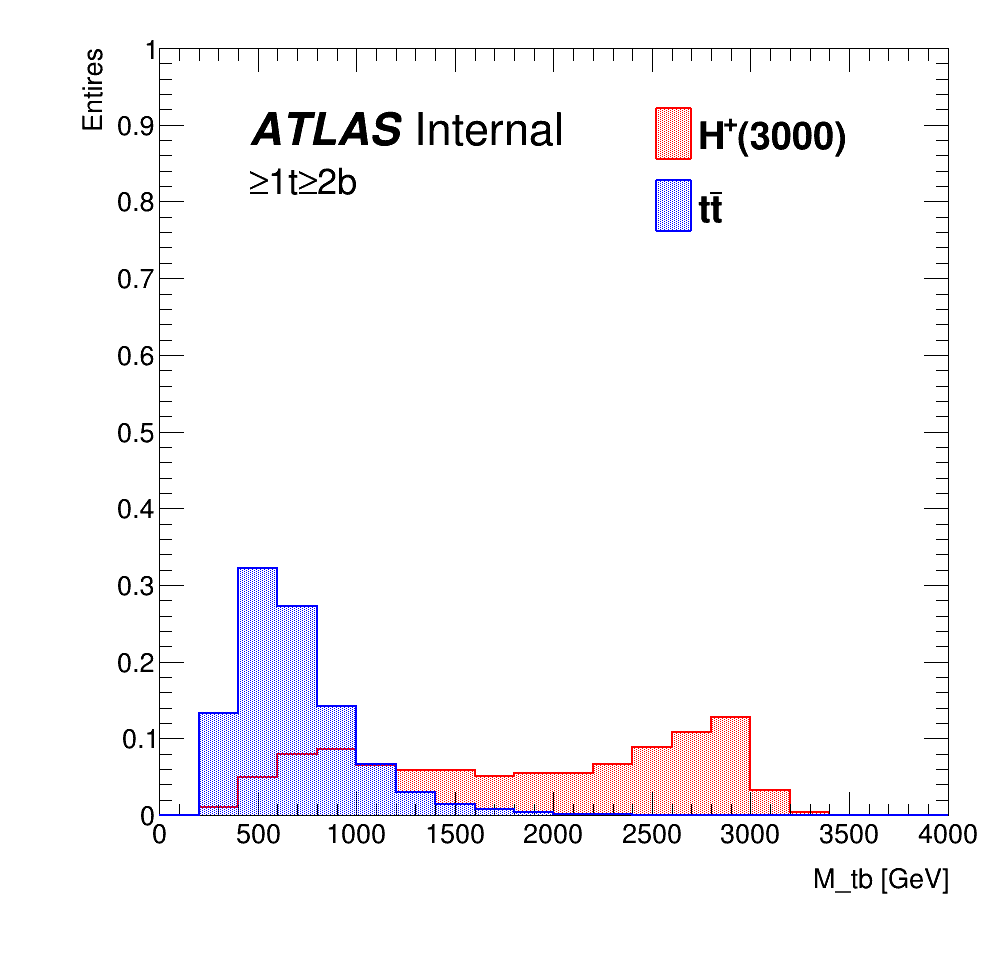
\includegraphics[width=0.25\textwidth]{images/AnalysisStrategy/SOVERB_Hp3000_Contained80_DL1r_70_tb_m_Contained80_DL1r_70.png}
        \label{fig:SOVERB_M_tb_Hp3000_Contained80_DL1r_70}
      }\\
      \subfloat[Pt\_tb] {
        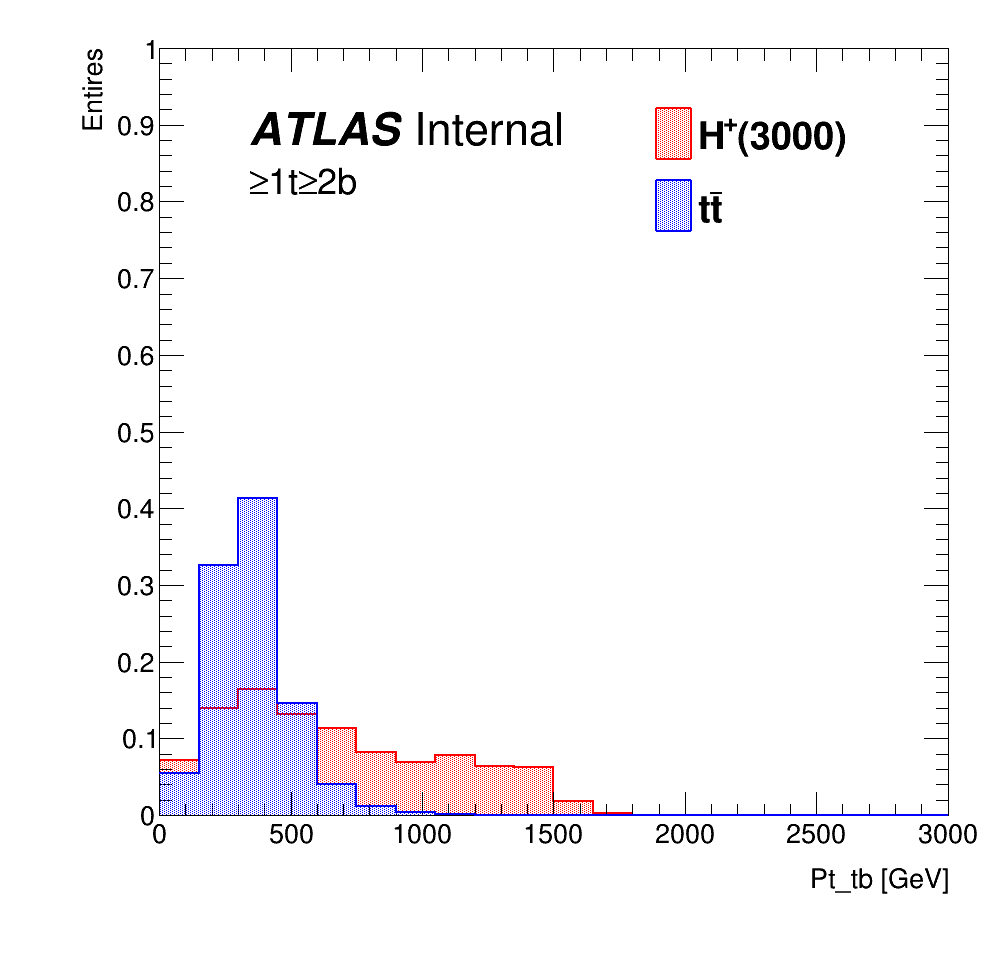
\includegraphics[width=0.25\textwidth]{images/AnalysisStrategy/SOVERB_Hp3000_Contained80_DL1r_70_tb_pt_Contained80_DL1r_70.png}
        \label{fig:SOVERB_Pt_tb_Hp3000_Contained80_DL1r_70}
      }
      \caption{Comparison of input variables for BDT training between $H^{+}$ and $t\bar{t}+\text{jets}$ events under 3000 GeV $H^{+}$ mass hypothesis in the SR.}
      \label{fig:SOVERB_Hp3000_Contained80_DL1r_70}
    \end{figure}

    \item{\textbf{Results of BDT training}}\mbox{}\\
    The BDT output distributions for $H^{+}$ signal and background events in the SR for different values of the $H^+$ mass are shown in Figure \ref{fig:BDTTrainingResults_Hp1000} to \ref{fig:BDTTrainingResults_Hp3000}, together with receiver operating characteristic (ROC) curves.

    %--- BDT template H+(1000)
    \begin{figure}[H]
      \centering
      \subfloat[BDT output]{
        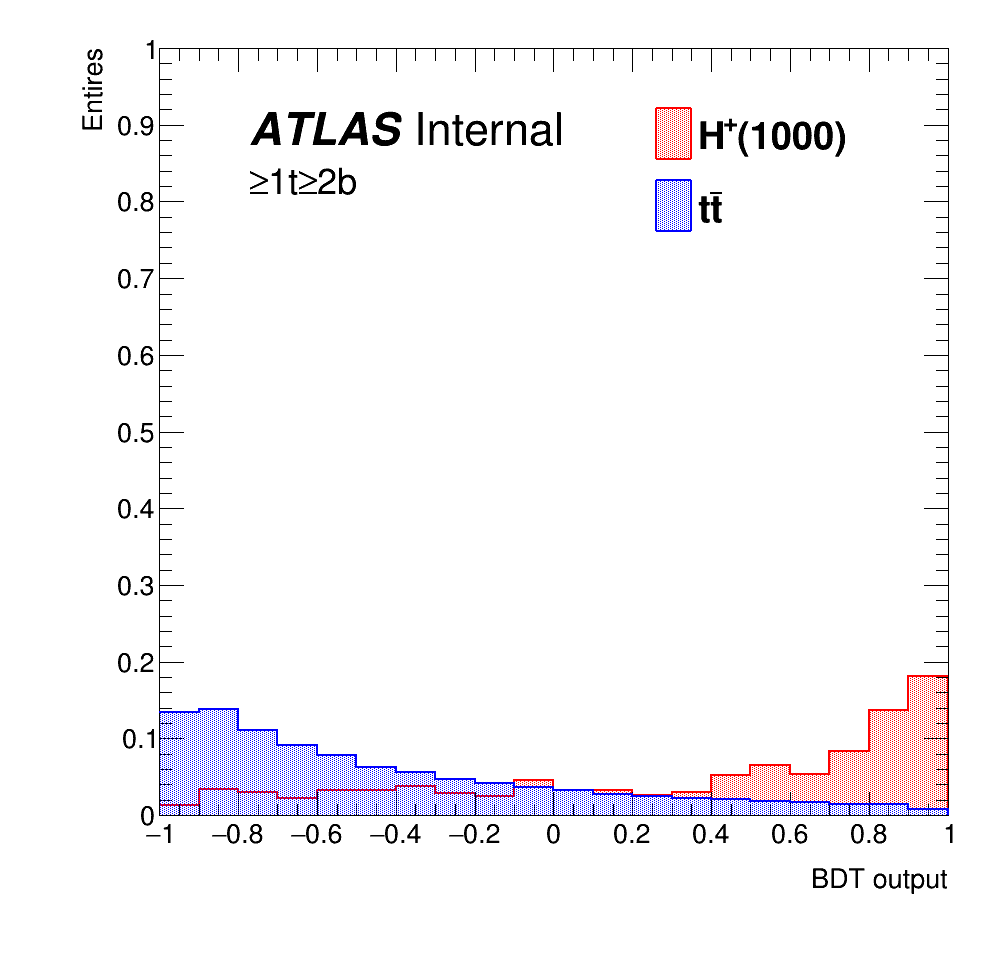
\includegraphics[width=0.45\textwidth]{images/AnalysisStrategy/BDTOutput_Hp1000_Contained80_DL1r_70.png}
        \label{fig:BDTOutput_Hp1000}
      }
      \subfloat[ROC curve]{
        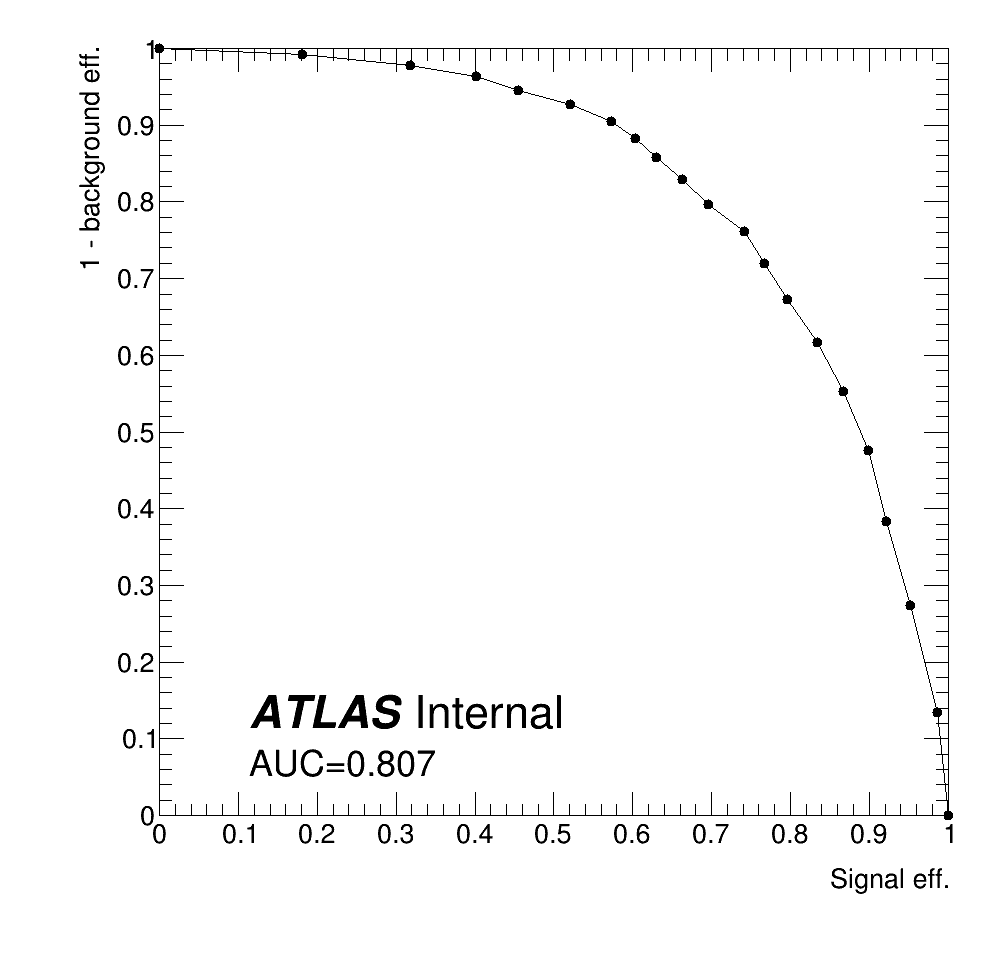
\includegraphics[width=0.45\textwidth]{images/AnalysisStrategy/ROCCurve_Hp1000_Contained80_DL1r_70.png}
        \label{fig:ROCCurve_Hp1000}
      }
      \caption{BDT distribution and ROC curve for the 1000 GeV $H^{+}$ mass hypothesis.}
      \label{fig:BDTTrainingResults_Hp1000}
    \end{figure}
    
    %--- BDT template H+(1200)
    \begin{figure}[H]
      \centering
      \subfloat[BDT output]{
        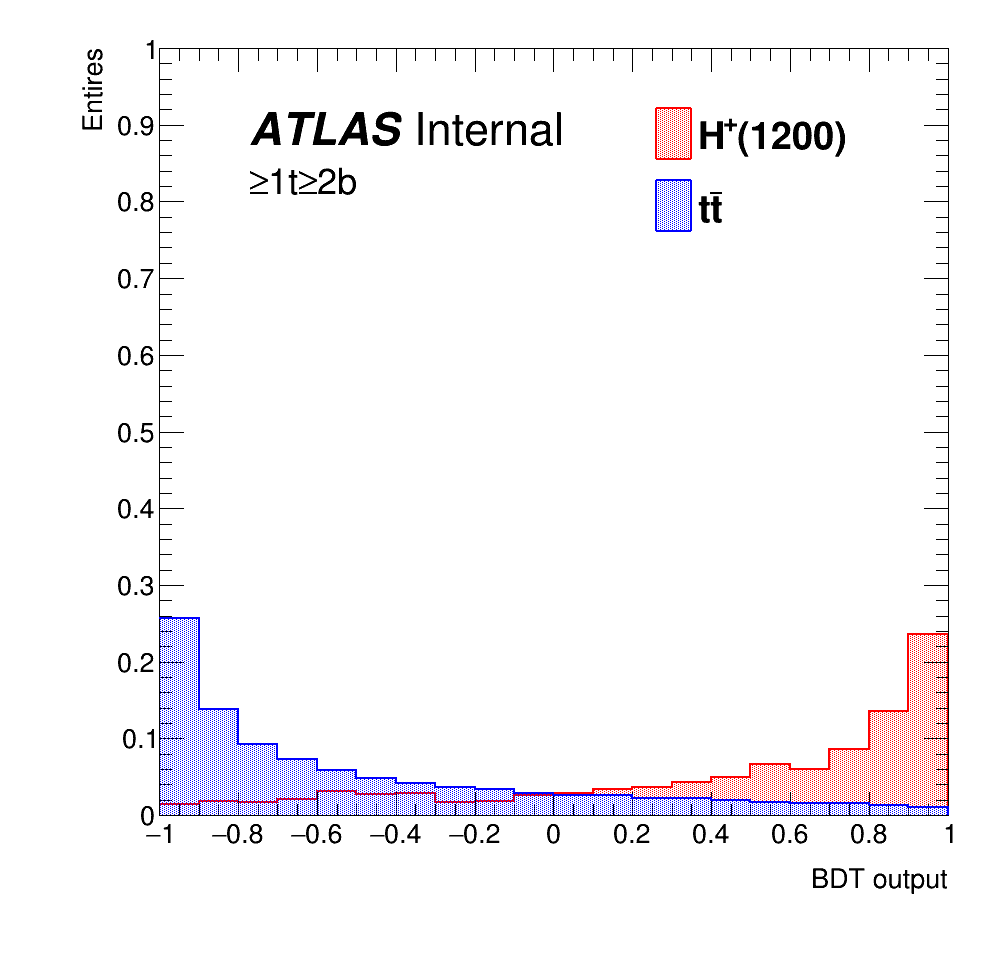
\includegraphics[width=0.45\textwidth]{images/AnalysisStrategy/BDTOutput_Hp1200_Contained80_DL1r_70.png}
        \label{fig:BDTOutput_Hp1200}
      }
      \subfloat[ROC curve]{
        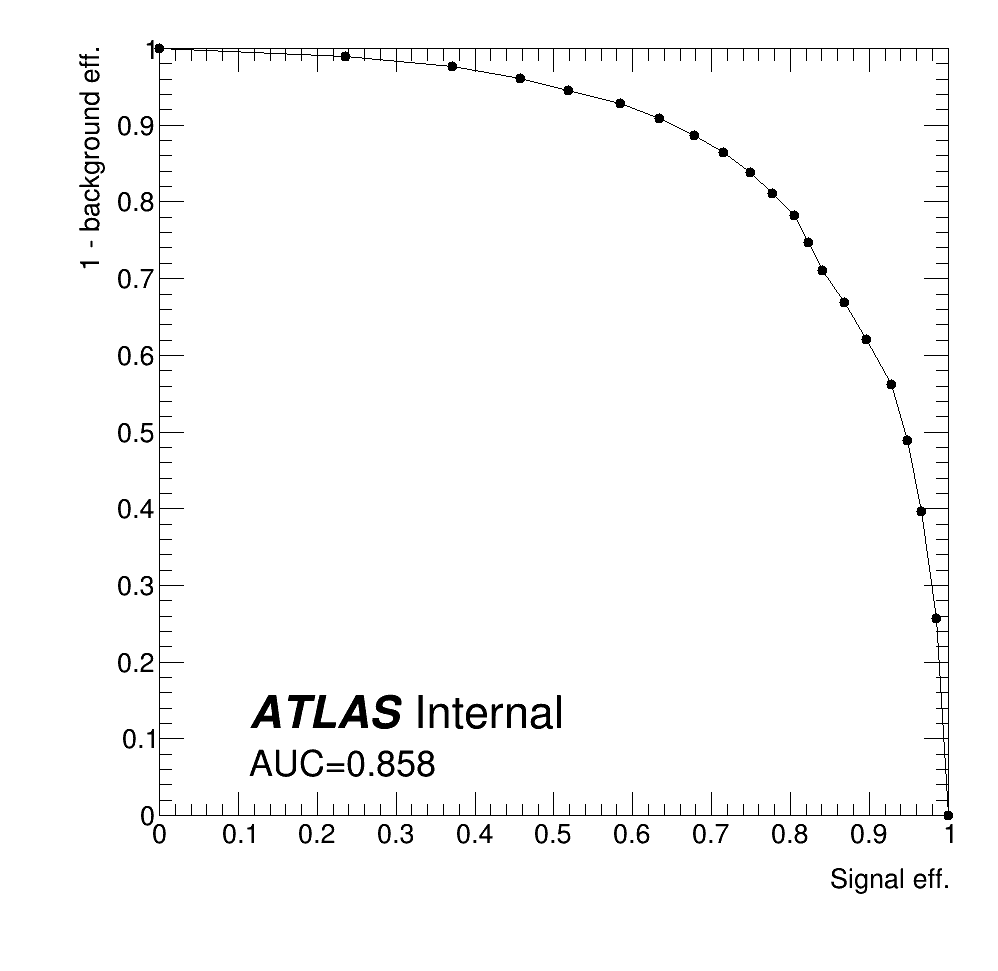
\includegraphics[width=0.45\textwidth]{images/AnalysisStrategy/ROCCurve_Hp1200_Contained80_DL1r_70.png}
        \label{fig:ROCCurve_Hp1200}
      }
      \caption{BDT distribution and ROC curve for the 1200 GeV $H^{+}$ mass hypothesis.}
      \label{fig:BDTTrainingResults_Hp1200}
    \end{figure}
    
    %--- BDT template H+(1400)
    \begin{figure}[H]
      \centering
      \subfloat[BDT output]{
        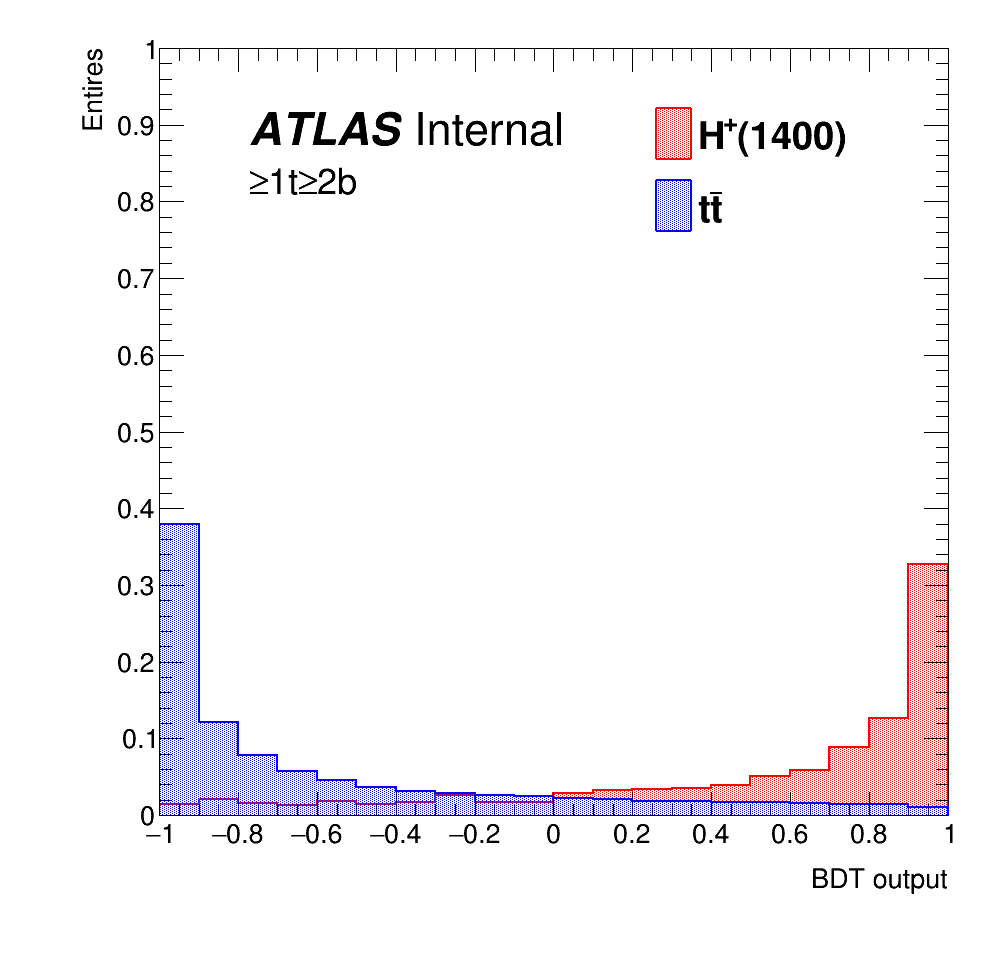
\includegraphics[width=0.45\textwidth]{images/AnalysisStrategy/BDTOutput_Hp1400_Contained80_DL1r_70.png}
        \label{fig:BDTOutput_Hp1400}
      }
      \subfloat[ROC curve]{
        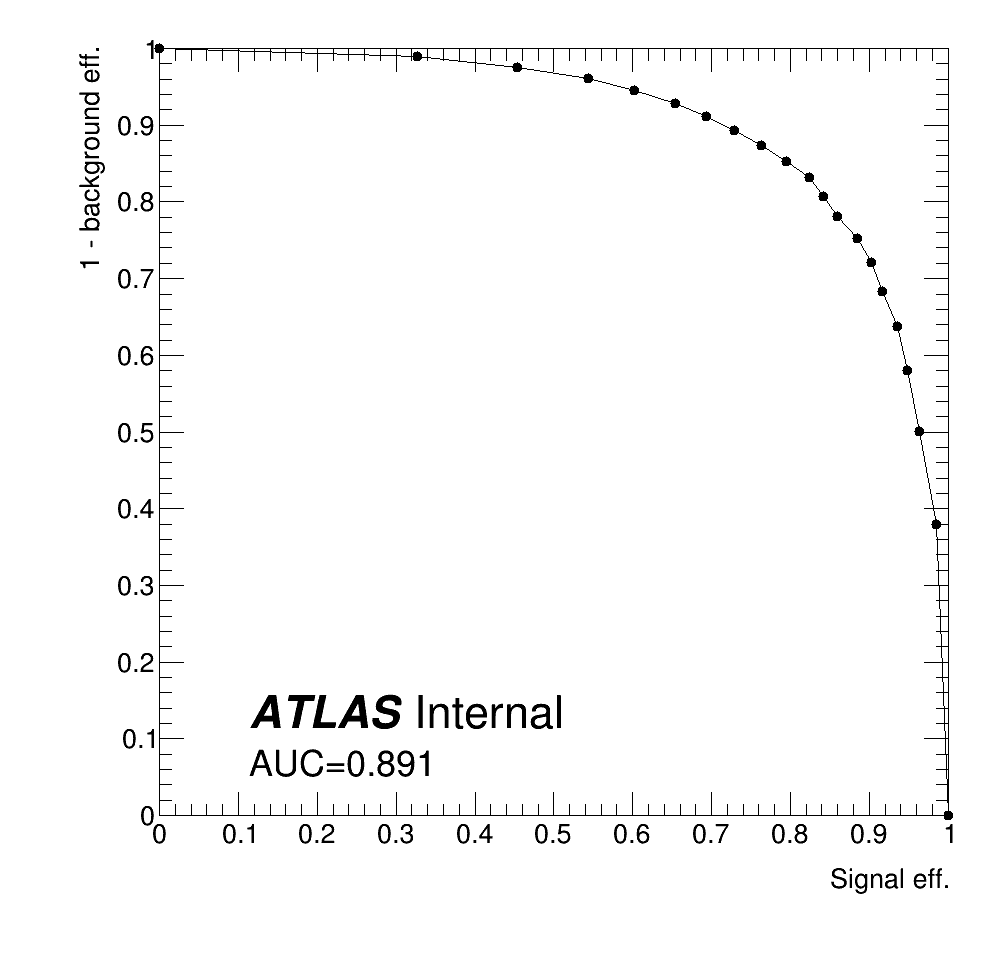
\includegraphics[width=0.45\textwidth]{images/AnalysisStrategy/ROCCurve_Hp1400_Contained80_DL1r_70.png}
        \label{fig:ROCCurve_Hp1400}
      }
      \caption{BDT distribution and ROC curve for the 1400 GeV $H^{+}$ mass hypothesis.}
      \label{fig:BDTTrainingResults_Hp1400}
    \end{figure}
    
    %--- BDT template H+(1600)
    \begin{figure}[H]
      \centering
      \subfloat[BDT output]{
        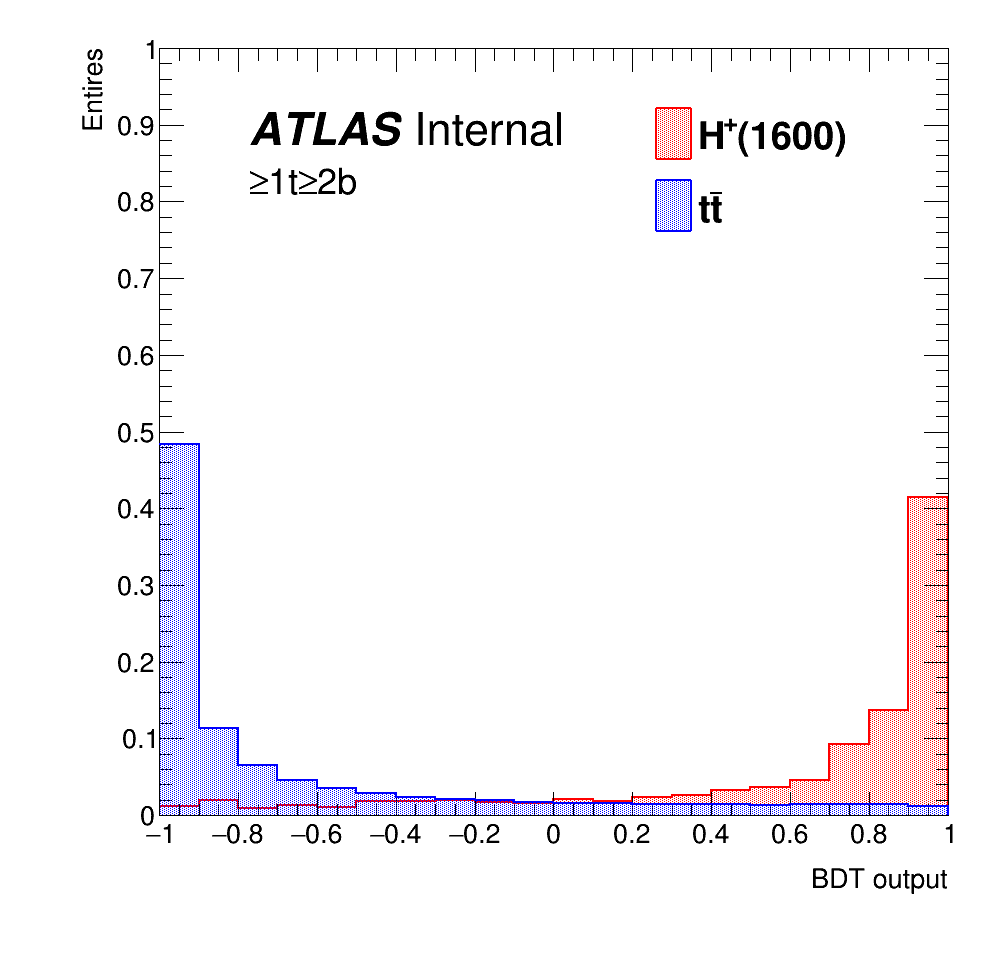
\includegraphics[width=0.45\textwidth]{images/AnalysisStrategy/BDTOutput_Hp1600_Contained80_DL1r_70.png}
        \label{fig:BDTOutput_Hp1600}
      }
      \subfloat[ROC curve]{
        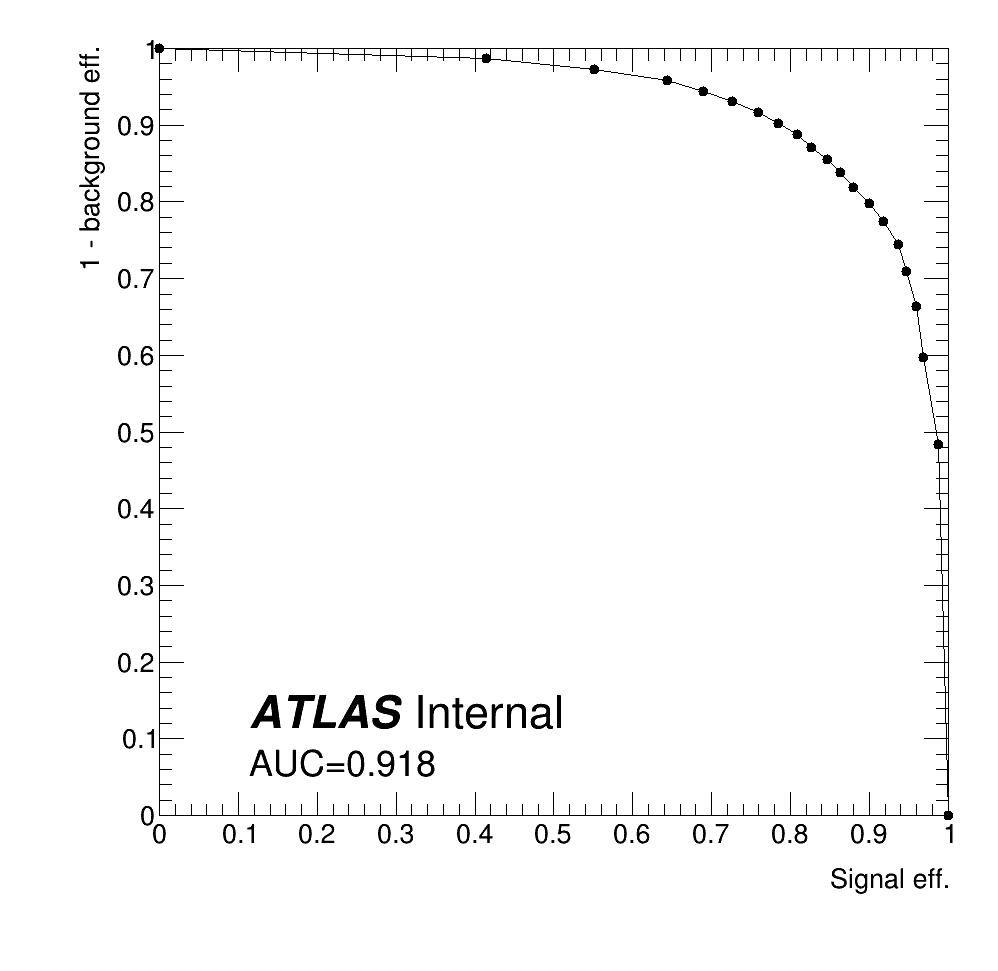
\includegraphics[width=0.45\textwidth]{images/AnalysisStrategy/ROCCurve_Hp1600_Contained80_DL1r_70.png}
        \label{fig:ROCCurve_Hp1600}
      }
      \caption{BDT distribution and ROC curve for the 1600 GeV $H^{+}$ mass hypothesis.}
      \label{fig:BDTTrainingResults_Hp1600}
    \end{figure}
    
    %--- BDT template H+(1800)
    \begin{figure}[H]
      \centering
      \subfloat[BDT output]{
        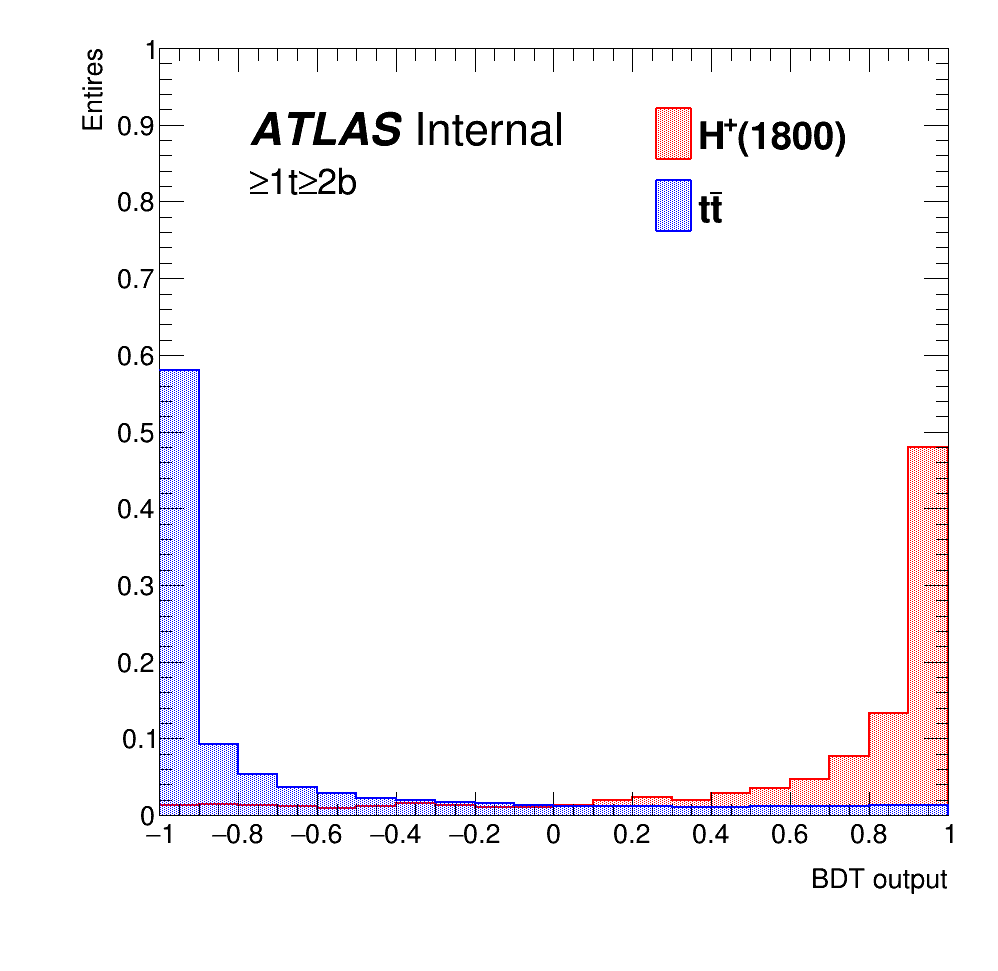
\includegraphics[width=0.45\textwidth]{images/AnalysisStrategy/BDTOutput_Hp1800_Contained80_DL1r_70.png}
        \label{fig:BDTOutput_Hp1800}
      }
      \subfloat[ROC curve]{
        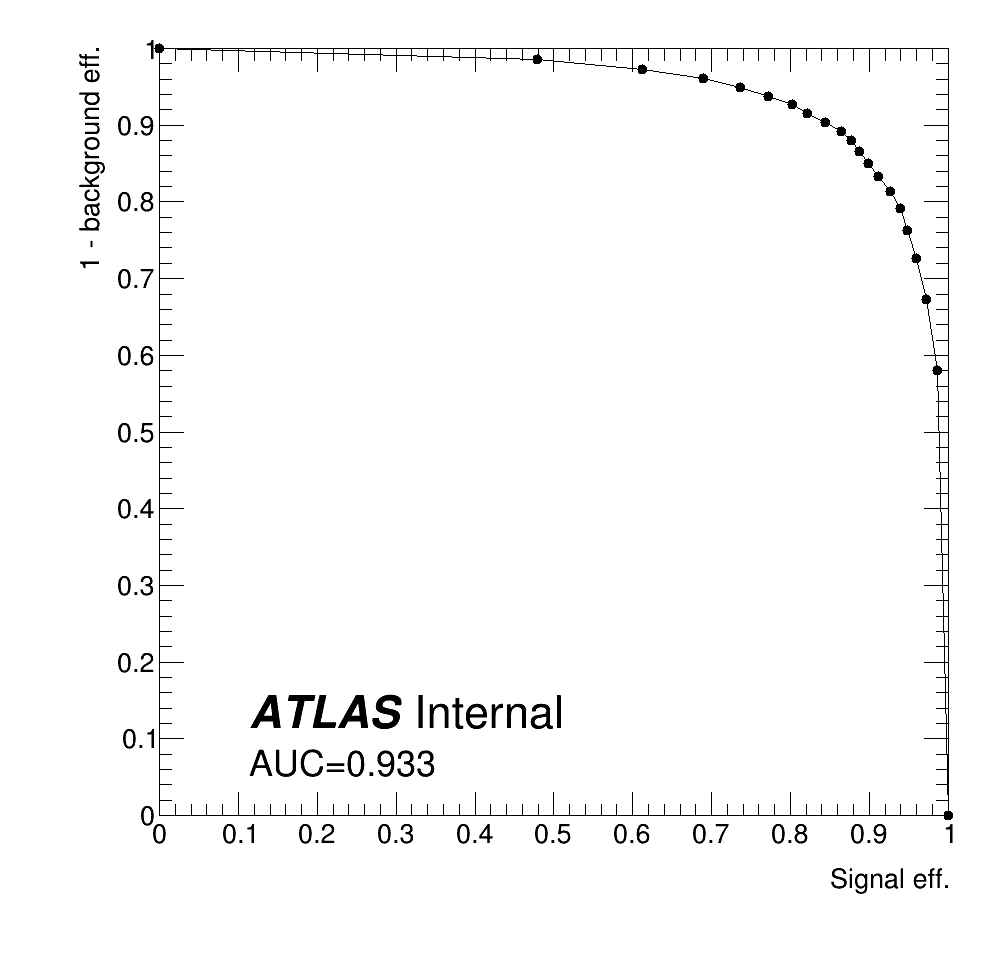
\includegraphics[width=0.45\textwidth]{images/AnalysisStrategy/ROCCurve_Hp1800_Contained80_DL1r_70.png}
        \label{fig:ROCCurve_Hp1800}
      }
      \caption{BDT distribution and ROC curve for the 1800 GeV $H^{+}$ mass hypothesis.}
      \label{fig:BDTTrainingResults_Hp1800}
    \end{figure}
    
    %--- BDT template H+(2000)
    \begin{figure}[H]
      \centering
      \subfloat[BDT output]{
        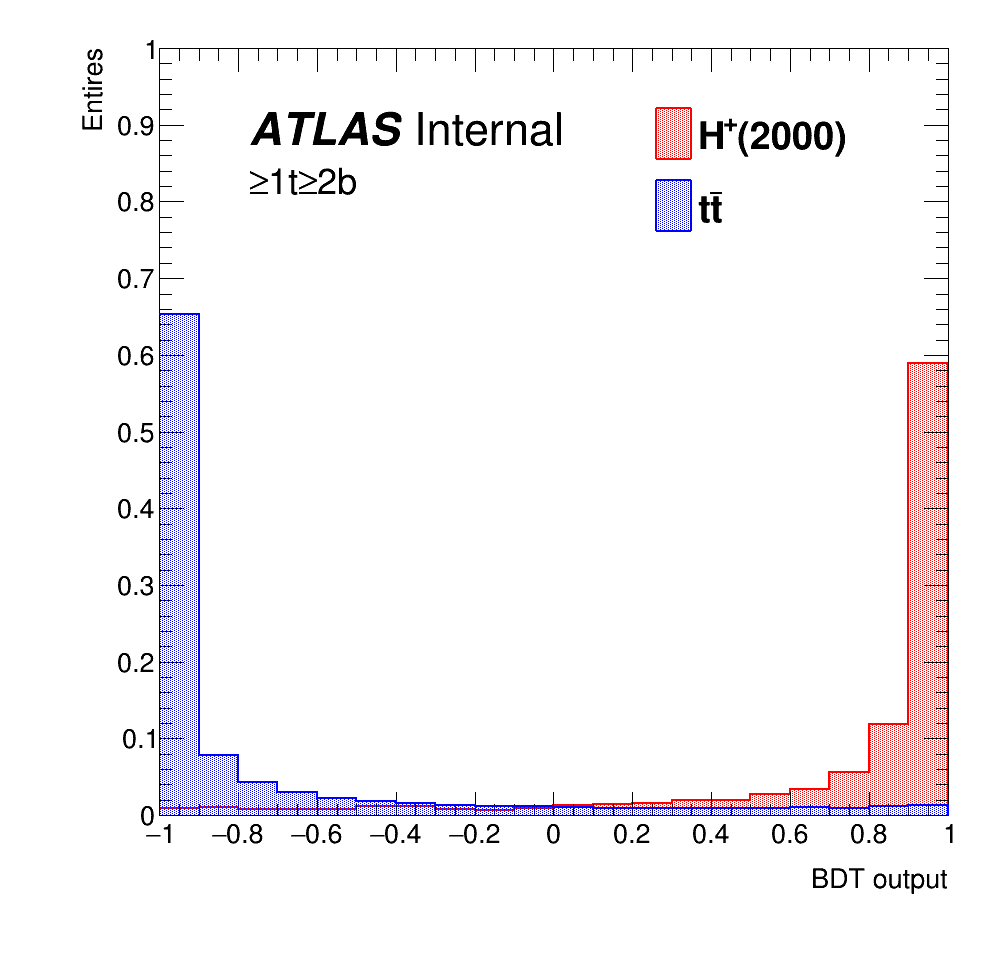
\includegraphics[width=0.45\textwidth]{images/AnalysisStrategy/BDTOutput_Hp2000_Contained80_DL1r_70.png}
        \label{fig:BDTOutput_Hp2000}
      }
      \subfloat[ROC curve]{
        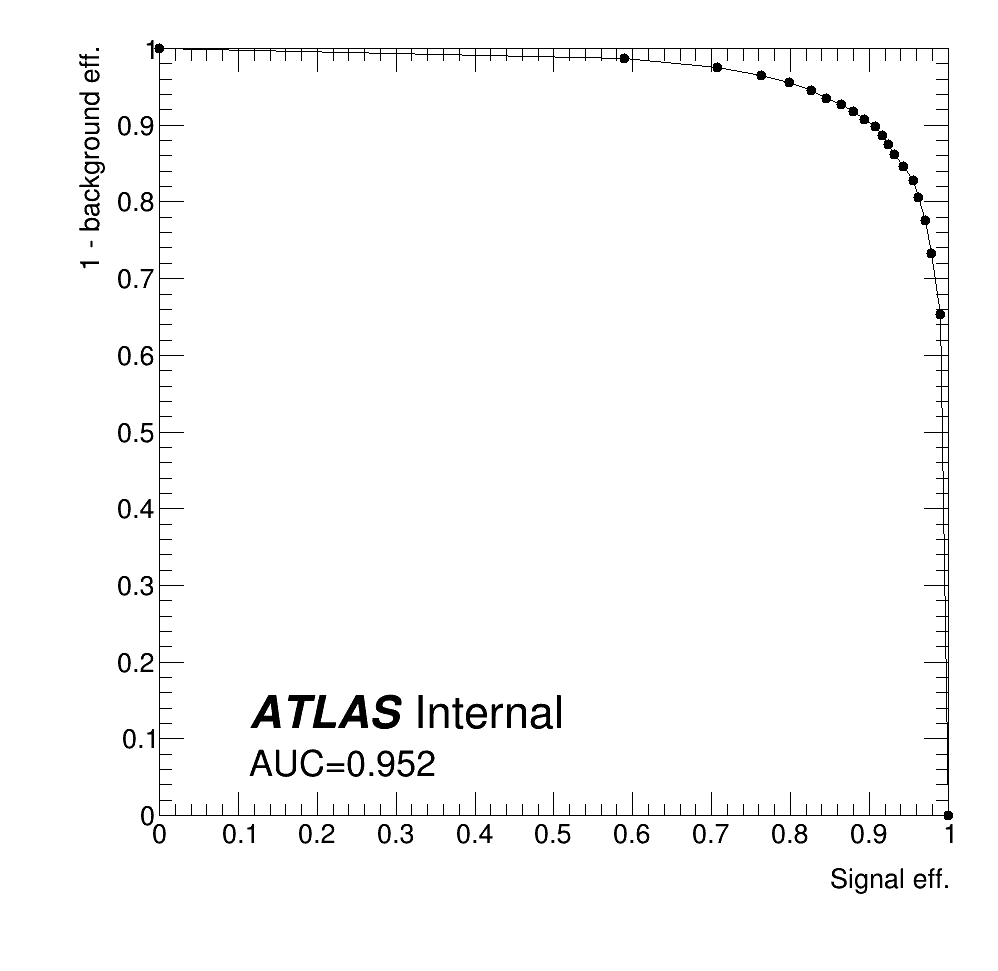
\includegraphics[width=0.45\textwidth]{images/AnalysisStrategy/ROCCurve_Hp2000_Contained80_DL1r_70.png}
        \label{fig:ROCCurve_Hp2000}
      }
      \caption{BDT distribution and ROC curve for the 2000 GeV $H^{+}$ mass hypothesis.}
      \label{fig:BDTTrainingResults_Hp2000}
    \end{figure}
    
    %--- BDT template H+(2500)
    \begin{figure}[H]
      \centering
      \subfloat[BDT output]{
        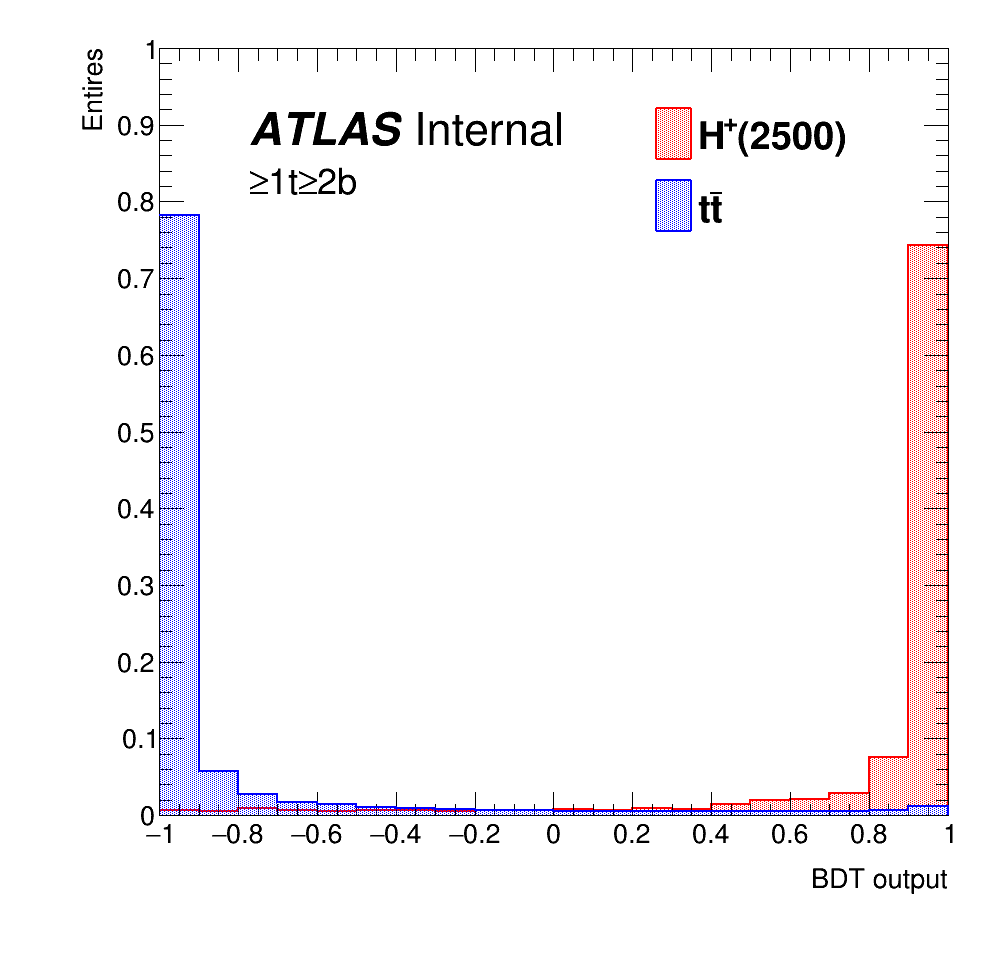
\includegraphics[width=0.45\textwidth]{images/AnalysisStrategy/BDTOutput_Hp2500_Contained80_DL1r_70.png}
        \label{fig:BDTOutput_Hp2500}
      }
      \subfloat[ROC curve]{
        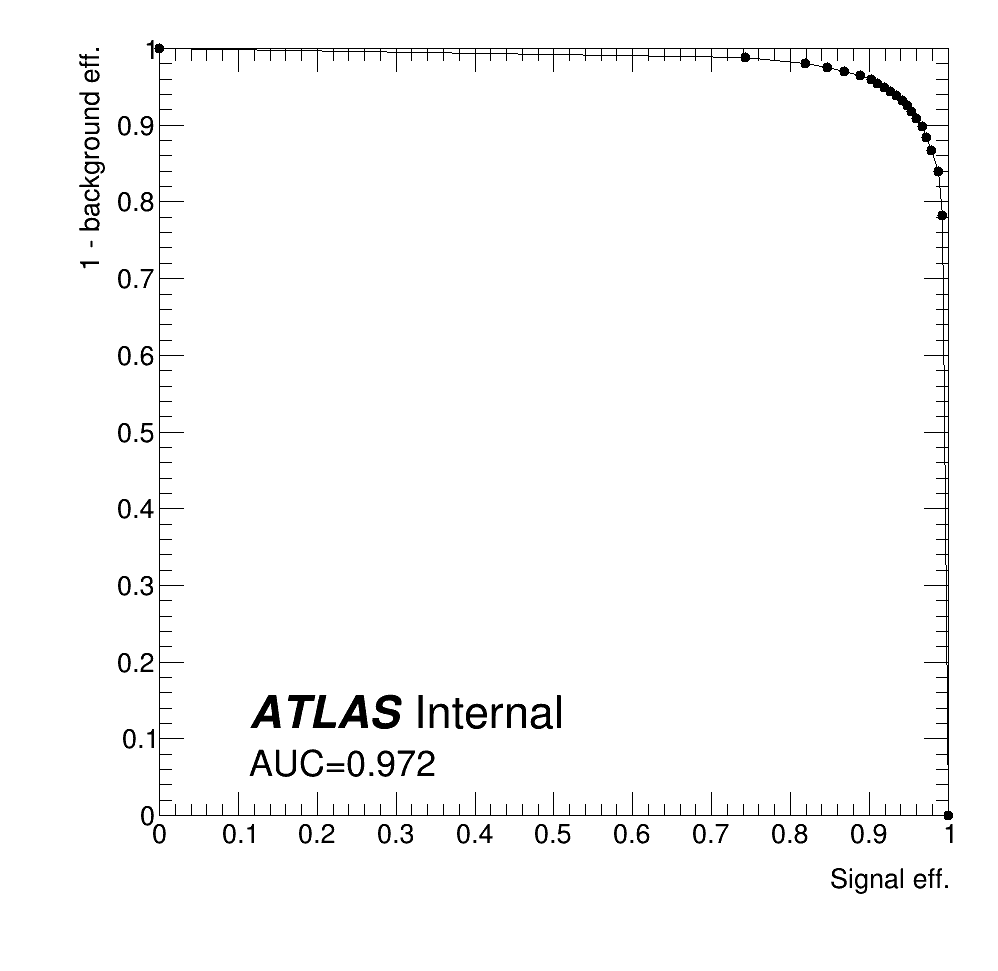
\includegraphics[width=0.45\textwidth]{images/AnalysisStrategy/ROCCurve_Hp2500_Contained80_DL1r_70.png}
        \label{fig:ROCCurve_Hp2500}
      }
      \caption{BDT distribution and ROC curve for the 2500 GeV $H^{+}$ mass hypothesis.}
      \label{fig:BDTTrainingResults_Hp2500}
    \end{figure}
    
    %--- BDT template H+(3000)
    \begin{figure}[H]
      \centering
      \subfloat[BDT output]{
        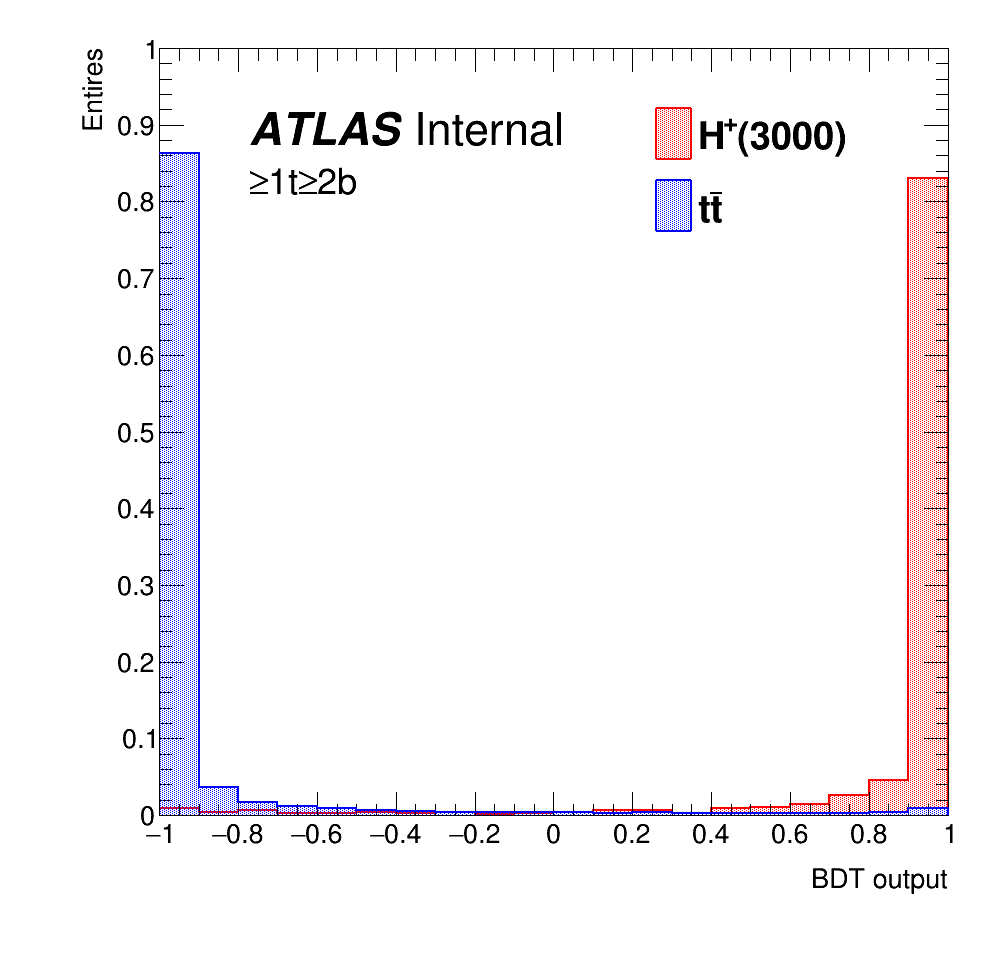
\includegraphics[width=0.45\textwidth]{images/AnalysisStrategy/BDTOutput_Hp3000_Contained80_DL1r_70.png}
        \label{fig:BDTOutput_Hp3000}
      }
      \subfloat[ROC curve]{
        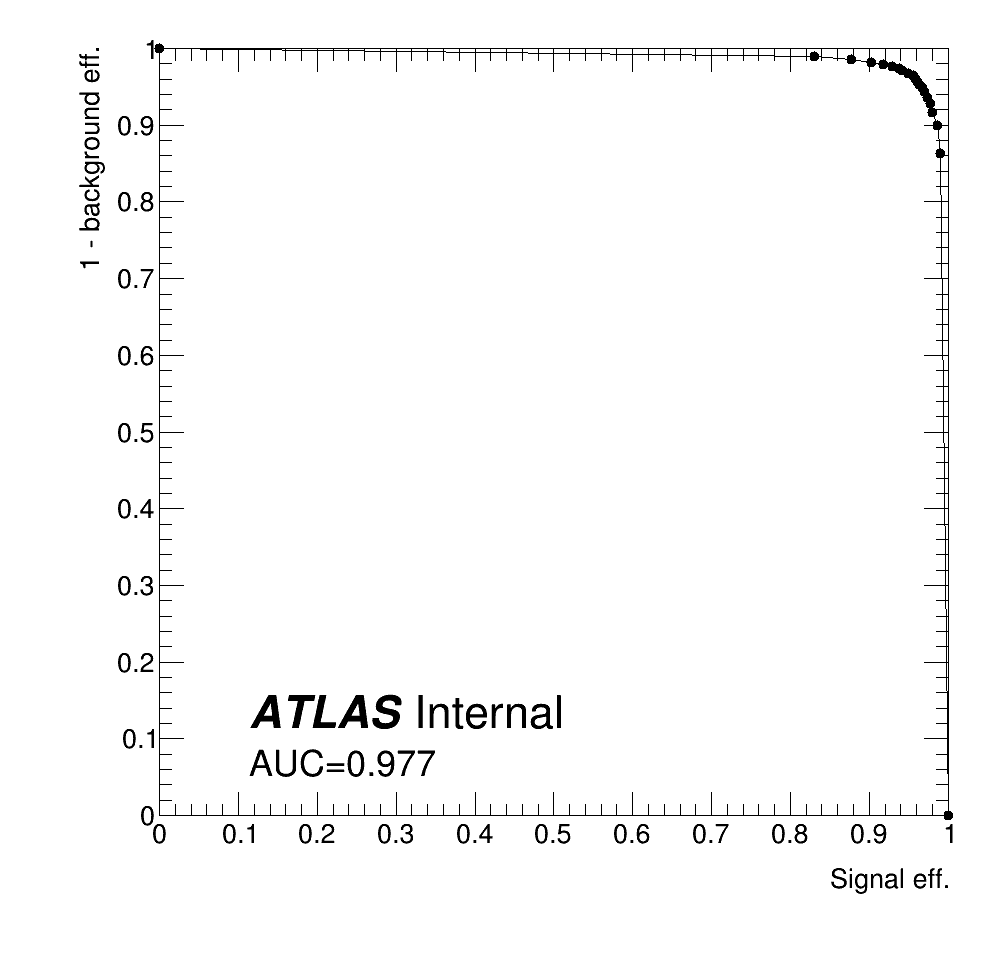
\includegraphics[width=0.45\textwidth]{images/AnalysisStrategy/ROCCurve_Hp3000_Contained80_DL1r_70.png}
        \label{fig:ROCCurve_Hp3000}
      }
      \caption{BDT distribution and ROC curve for the 3000 GeV $H^{+}$ mass hypothesis.}
      \label{fig:BDTTrainingResults_Hp3000}
    \end{figure}

    \item{\textbf{Comparison of BDT distributions between $H^{+} \rightarrow tb$ and  $W' \rightarrow tb$ events}}\mbox{}\\
    BDT distributions for $W' \rightarrow tb$ events are compared with the ones for $H^{+} \rightarrow tb$ events in Figure \ref{fig:CompHpAndWp}. The large differences above their statistic uncertainty are not observed. Therefore, it is expected to be able to obtain comparable sensitivity with $H^{+} \rightarrow tb$ analysis without further optimization using $W' \rightarrow tb$ samples.

    %--- Comparison of BDT outputs between H+ and W'
    \begin{figure}[H]
        \centering
        \subfloat[$M=1.0$ TeV]{
            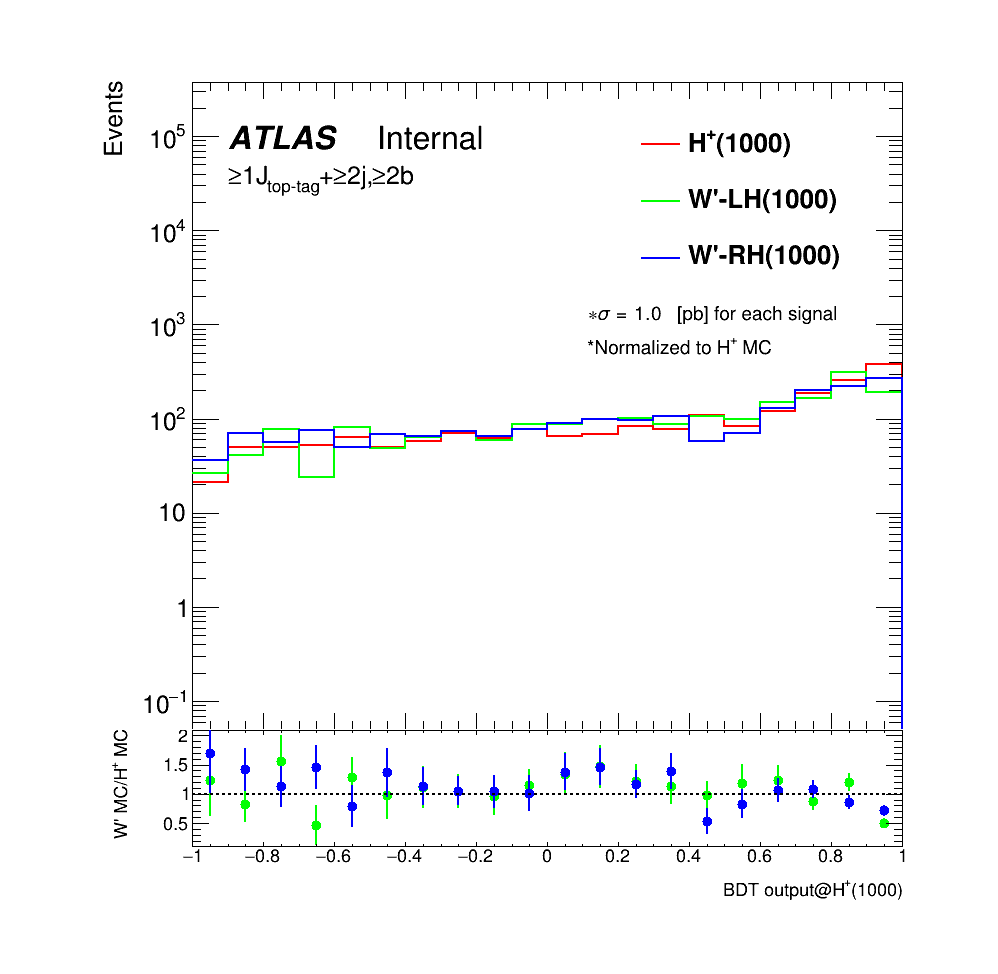
\includegraphics[width=0.45\textwidth]{images/AnalysisStrategy/bdt_Hp1000_1000_geq1tgeq2jgeq2b.png}
            \label{fig:CompHpAndWp_M1000}
        }
        \subfloat[$M=1.2$ TeV]{
            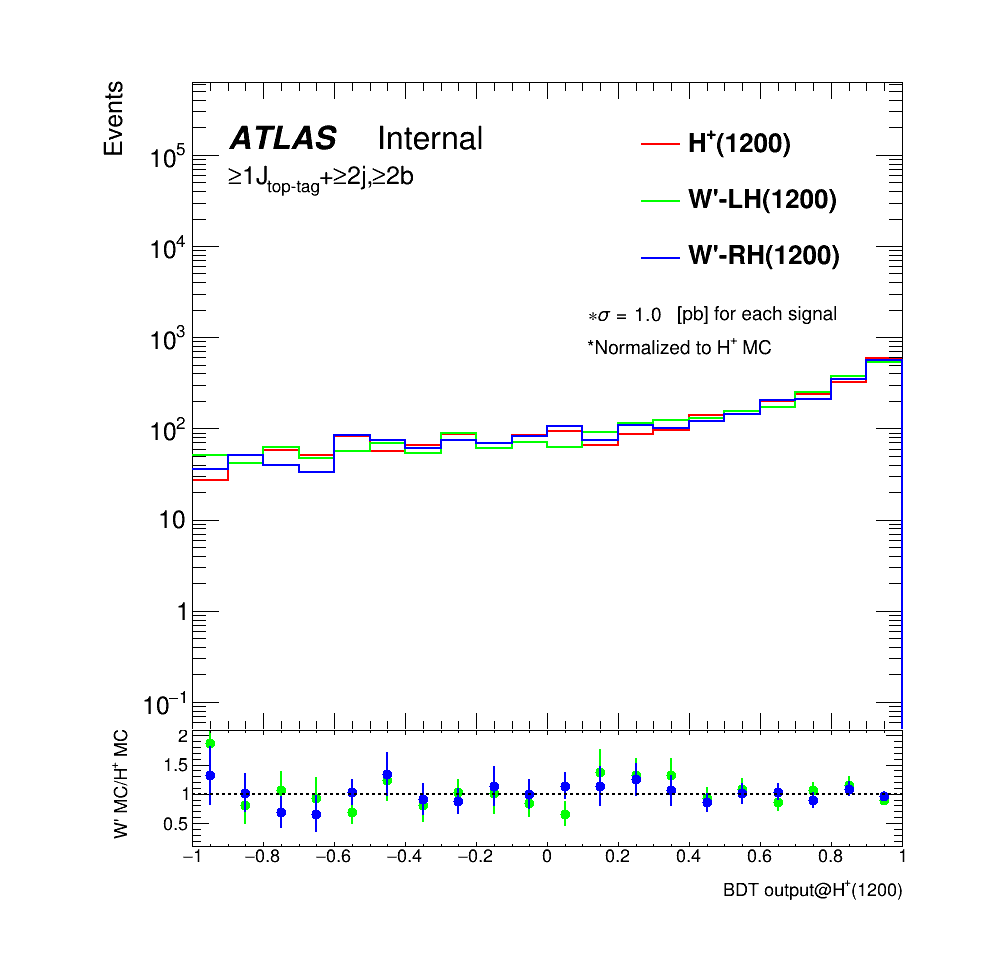
\includegraphics[width=0.45\textwidth]{images/AnalysisStrategy/bdt_Hp1200_1200_geq1tgeq2jgeq2b.png}
            \label{fig:CompHpAndWp_M1200}
        }\\
        \subfloat[$M=1.4$ TeV]{
            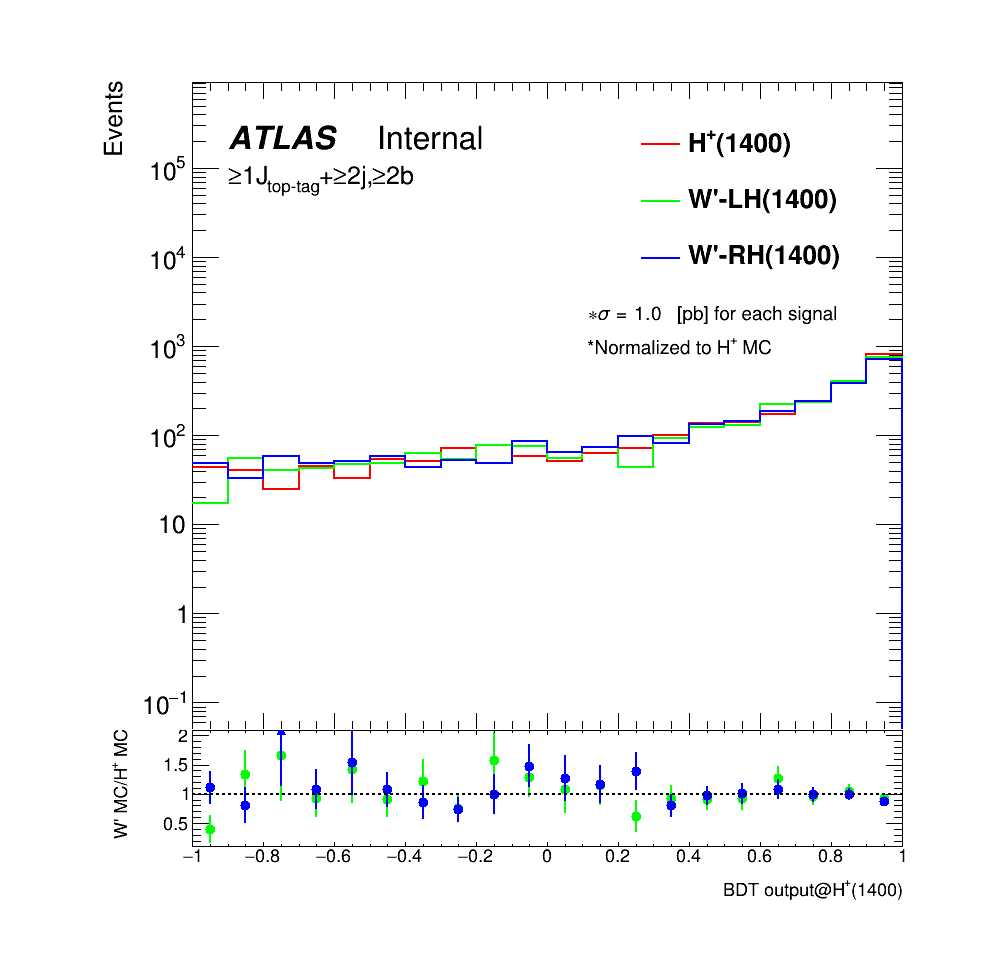
\includegraphics[width=0.45\textwidth]{images/AnalysisStrategy/bdt_Hp1400_1400_geq1tgeq2jgeq2b.png}
            \label{fig:CompHpAndWp_M1400}
        }  
        \subfloat[$M=1.6$ TeV]{
            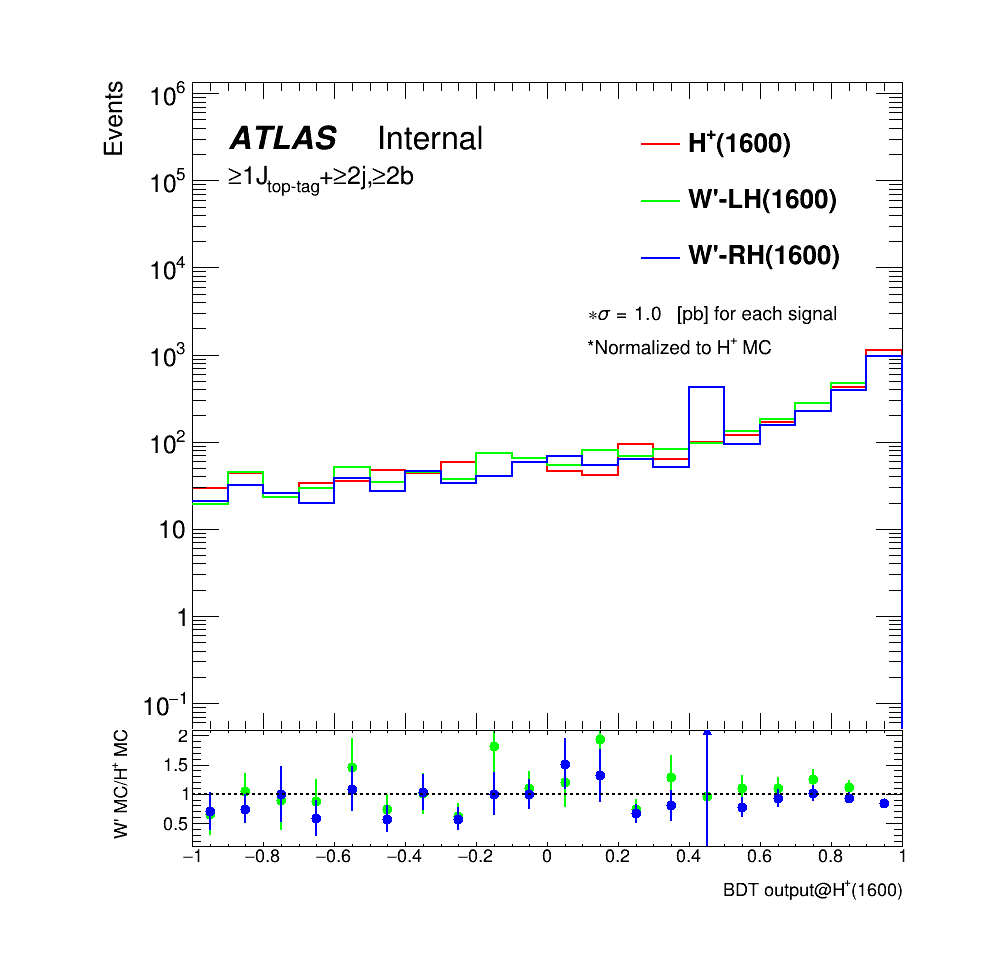
\includegraphics[width=0.45\textwidth]{images/AnalysisStrategy/bdt_Hp1600_1600_geq1tgeq2jgeq2b.png}
            \label{fig:CompHpAndWp_M1600}
        }\\
    \end{figure}
    \begin{figure}[H]
        %\addtocounter{figure}{-1}
        \subfloat[$M=1.8$ TeV]{
             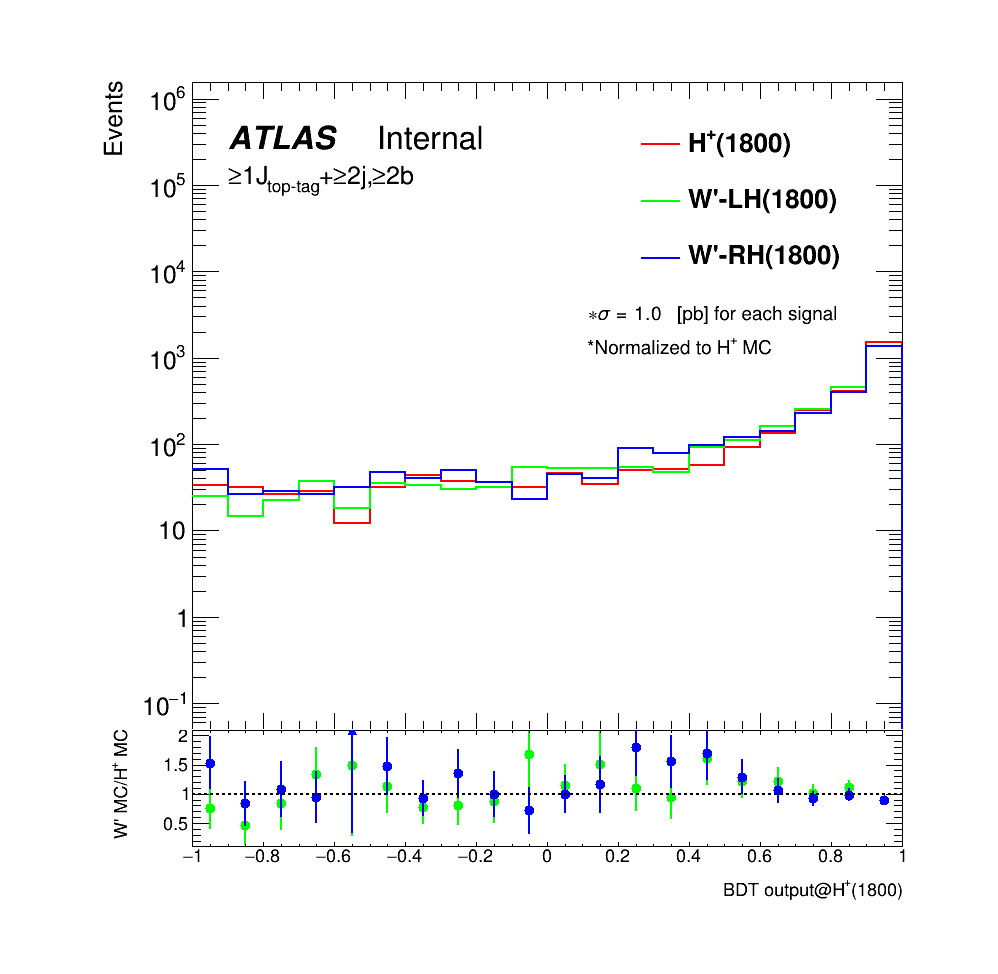
\includegraphics[width=0.45\textwidth]{images/AnalysisStrategy/bdt_Hp1800_1800_geq1tgeq2jgeq2b.png}
             \label{fig:CompHpAndWp_M1800}
        }
        \subfloat[$M=2.0$ TeV]{
            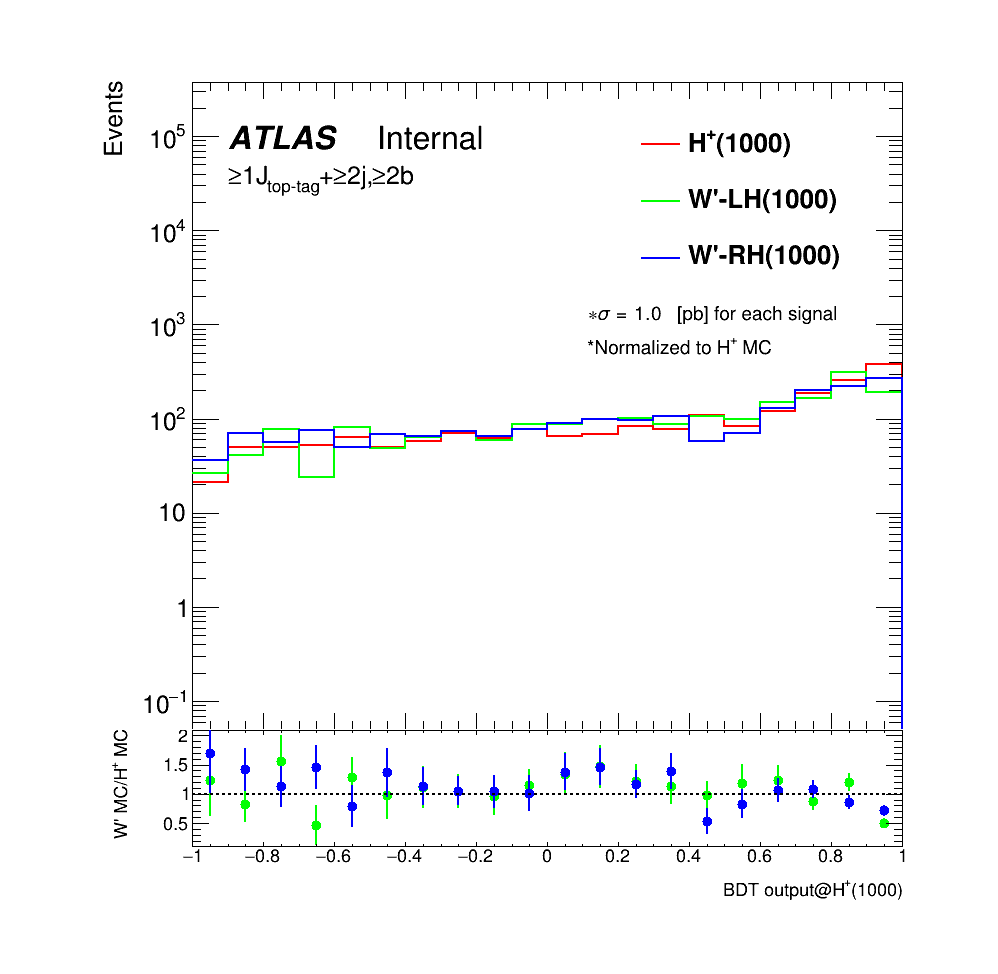
\includegraphics[width=0.45\textwidth]{images/AnalysisStrategy/bdt_Hp1000_1000_geq1tgeq2jgeq2b.png}
            \label{fig:CompHpAndWp_M2000}
        }\\
        \subfloat[$M=2.5$ TeV]{
            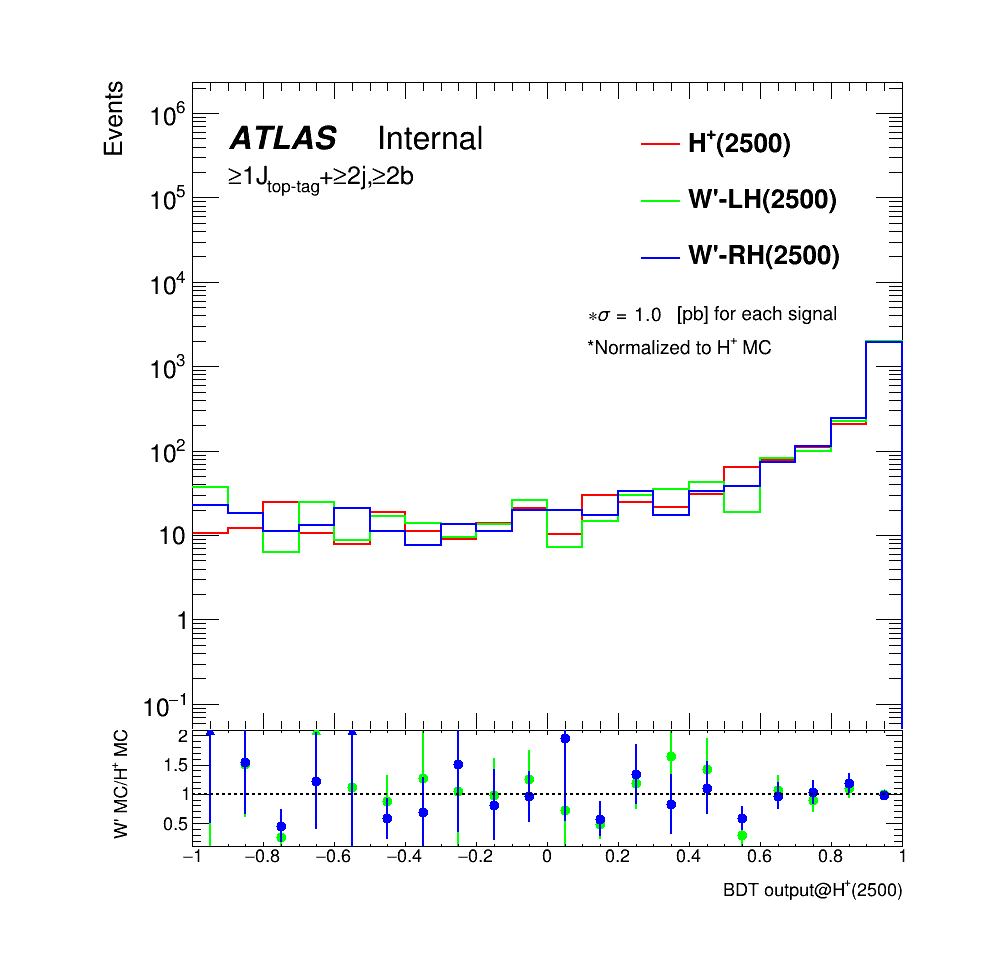
\includegraphics[width=0.45\textwidth]{images/AnalysisStrategy/bdt_Hp2500_2500_geq1tgeq2jgeq2b.png}
            \label{fig:CompHpAndWp_M2500}
        }  
        \subfloat[$M=3.0$ TeV]{
            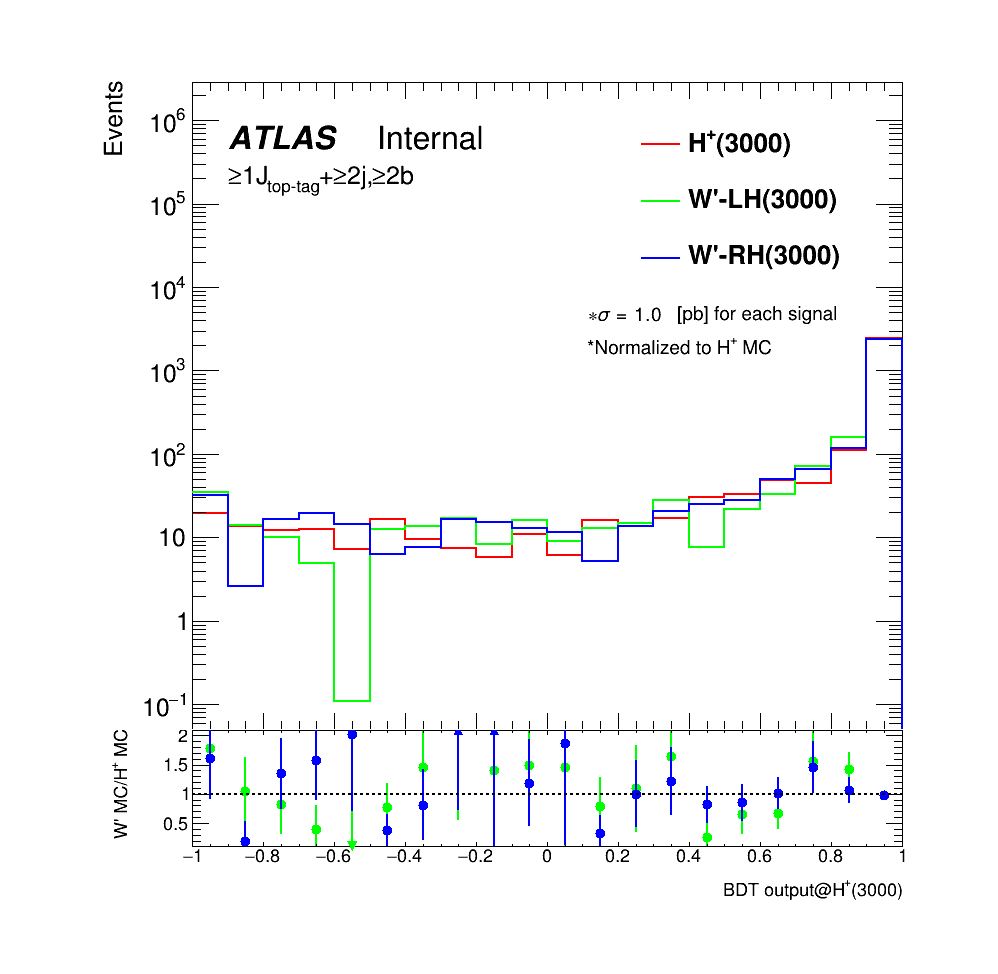
\includegraphics[width=0.45\textwidth]{images/AnalysisStrategy/bdt_Hp3000_3000_geq1tgeq2jgeq2b.png}
            \label{fig:CompHpAndWp_M3000}
        }
        \caption{Comparison of BDT distributions between $H^{+} \rightarrow tb$ and  $W' \rightarrow tb$ events in the SR.}
        \label{fig:CompHpAndWp}
    \end{figure}
    
\end{description}

\subsection{Analysis strategy above 3 TeV}
\label{subsec:AnaStrategyAbove3TeV}
For the mass point above 3 TeV, we adopt a different approach. Since it is difficult to estimate $t\bar{t}+\text{jets}$ events reliably in the very high $H_{\text{T}}^{\text{jets}}$ region where most of the signal events distribute, we use a cut-and-counting method as detailed below, which avoids using the line shapes at the high $H_{\text{T}}^{\text{jets}}$ region, and therefore is more robust against potential mis-modelling compared with the BDT method. 

\begin{figure}[H]
    \subfloat[]{
        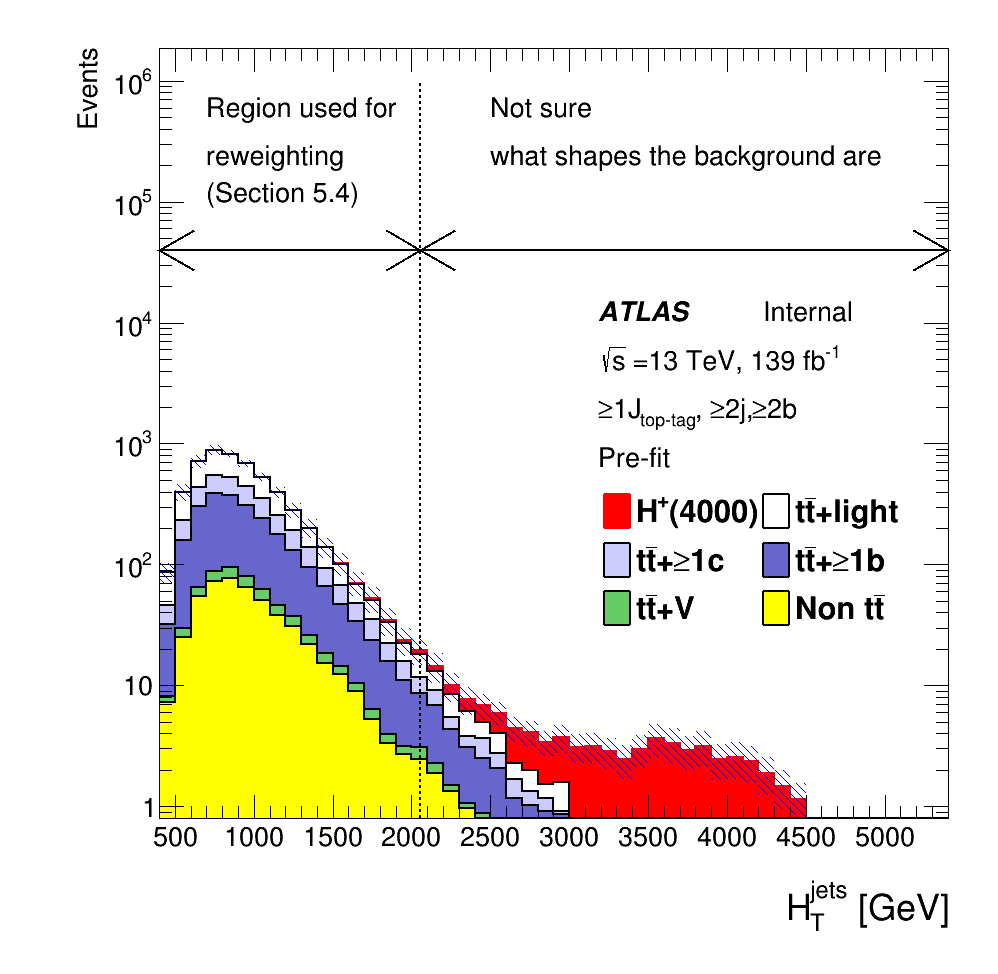
\includegraphics[width=0.45\textwidth]{images/AnalysisStrategy/SOVERB_Hp4000_Contained80_DL1r_70_HTjets_beforeRW_geq1tgeq2jgeq2b_prefit.png}
        \label{fig:SOVERB_HT_jets_4000GeV}
    }
    \subfloat[]{
        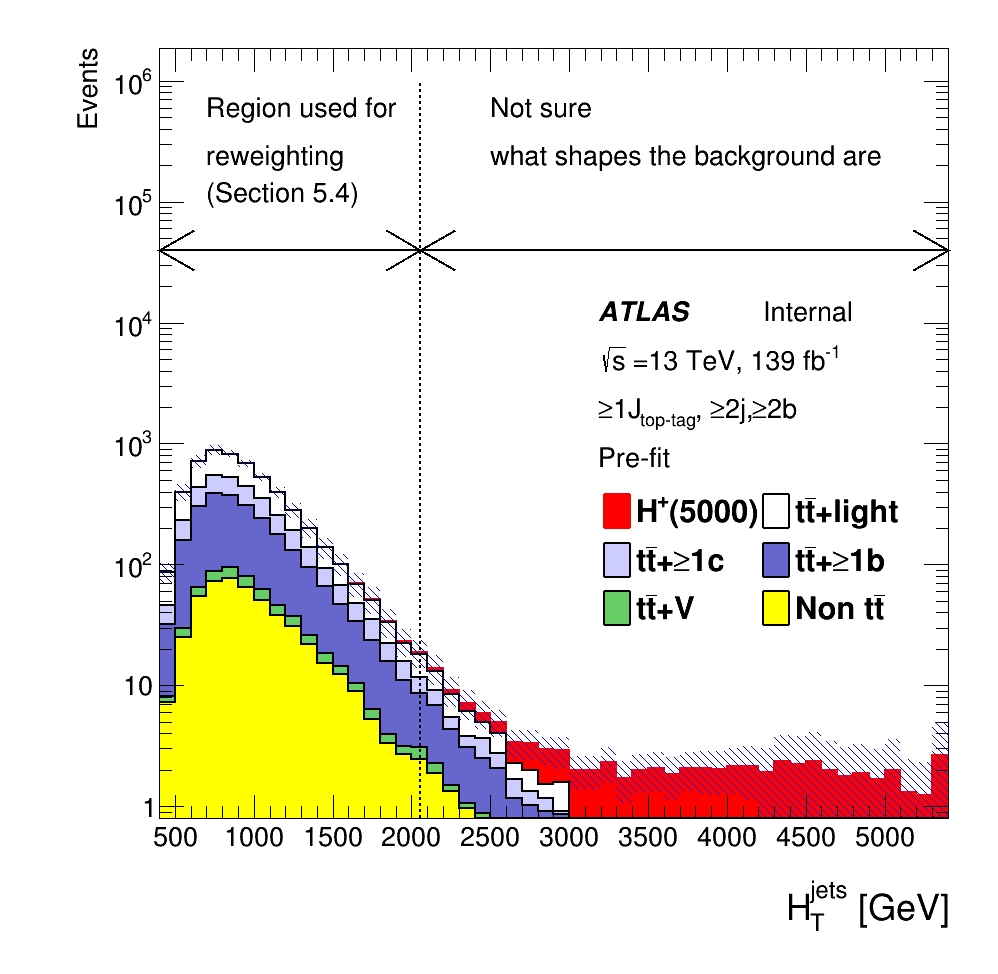
\includegraphics[width=0.45\textwidth]{images/AnalysisStrategy/SOVERB_Hp5000_Contained80_DL1r_70_HTjets_beforeRW_geq1tgeq2jgeq2b_prefit.png}
        \label{fig:SOVERB_HT_jets_5000GeV}
    }
    \caption{Signal and background comparison for 4000 (a) and 5000 (b) GeV mass hypotheses. These signal events distribute mostly in $H_{\text{T}}^{\text{jets}}>2000$ GeV. These regions don't have enough shape information to perform reweighting in Section \ref{subsec:ReweightingTechnique}.}
    \label{fig:SOVERB_HT_jets_4and5TeV}
\end{figure}

One signal region (SR) and two control regions (CR1, CR2) are defined according to the $H_{\text{T}}^{\text{jets}}$ and the number of $b$-jets. Events that have at least two $b$-tagged jets are first required to satisfy the same selection criteria for the SR of the multivariate analysis (Section \ref{subsubsec:RegionDefUnder3TeV}). They are categorized in the SR if they have $H_{\text{T}}^{\text{jets}}>2000$ GeV, while events with $H_{\text{T}}^{\text{jets}} \leq 2000$ are categorized into the CR1, depending on $\text{N}_{b_{\text{jets}}}$. All events that have exactly one $b$-tagged jet are categorized into CR2, which is the same as the CR of the multivariate analysis. The event selections in these regions are summarized in Table \ref{tab:EventSelectionInSRAndCR1AndCR2}. Figure \ref{fig:BkgComposition_SR_CC} to \ref{fig:BkgComposition_CR2_CC} shows the background compositions in each region. $H_{\text{T}}^{\text{jets}}$ is used as final discriminates, as discussed in Section \ref{sec:ProfileLikelohoodFit}. The number of bins of $H_{\text{T}}^{\text{jets}}$ distribution in the SR is set to one. The CR1 and CR2 are enriched in $t\bar{t}+\text{HF}$ and $t\bar{t}+\text{light}$ events, respectively. Therefore, these regions are used to control $t\bar{t}+\text{jets}$ events in the final fittings. 

\begin{table}[H]
    \centering
    \begin{tabular*}{130mm}{c|c|c|c}
        \hline\hline
        Cut                          & SR & CR1 & CR2\\
        \hline
        leptons                      & \multicolumn{3}{c}{Same requirements as Table \ref{tab:EventSelectionInSR1AndSR2}}\\
        \hline
        Top-tagged large-$R$ jets    & \multicolumn{3}{c}{Same requirements as Table \ref{tab:EventSelectionInSR1AndSR2}}\\
        \hline
        Small-$R$ jets               & \multicolumn{2}{c|}{$\text{N}_{\text{jet}} \geq 2$}    & $\text{N}_{\text{jet}} \geq 1$ \\
                                     & \multicolumn{2}{c|}{(Kinematic requirements}  & (Kinematic requirements \\
                                     & \multicolumn{2}{c|}{are the same as Table \ref{tab:EventSelectionInSR1AndSR2})} & are the same as Table \ref{tab:EventSelectionInSR1AndSR2})\\
        \hline
        $b$-tagged small-$R$ jets    & \multicolumn{2}{c|}{$\text{N}_{b-\text{jet}} \geq 2$}  & $\text{N}_{b-\text{jet}} = 1$\\
        \hline
        $H_{\text{T}}^{\text{jets}}$ & $> 2000$ GeV & $\leq 2000$ GeV & No cut\\
        \hline\hline
  \end{tabular*}
  \caption{Event selections in the SR, CR1, and CR2. After these selections, CR1 becomes enriched in $t\bar{t}+\text{light}$, and CR2 becomes enriched in $t\bar{t}+\text{HF}$.}
  \label{tab:EventSelectionInSRAndCR1AndCR2}
\end{table}

%--- Figure for SR
\begin{figure}[H]
  \centering
  \subfloat[]{
    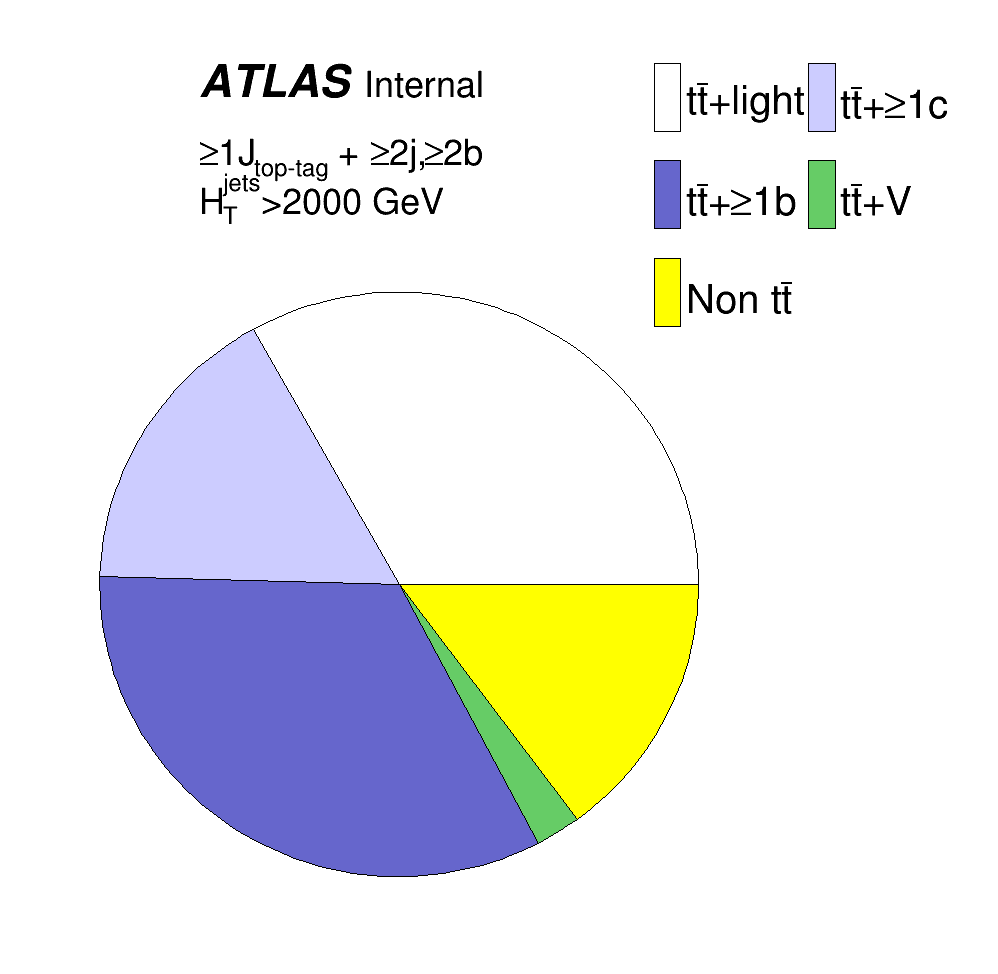
\includegraphics[keepaspectratio,scale=0.2]{images/AnalysisStrategy/PieChart_SR_CC.png}
    \label{fig:PieChart_SR_CC}
  }
  \subfloat[]{
    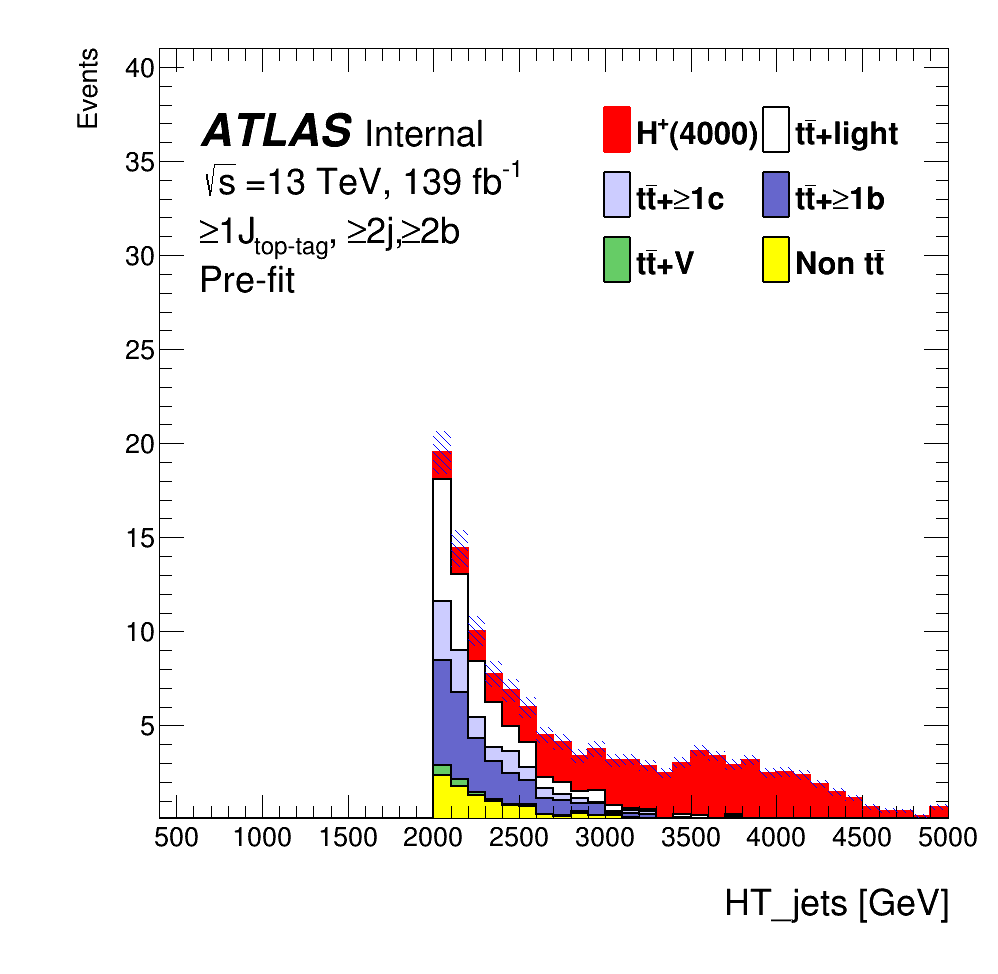
\includegraphics[keepaspectratio,scale=0.2]{images/AnalysisStrategy/HTjets_SR_CC.png}
    \label{fig:PieChart_SR1}
  }
  \caption{Background composition in the SR is shown in the pie chart (a) and the $H_{\text{T}}^{\text{jets}}$ distributions (b). The number of bins of $H_{\text{T}}^{\text{jets}}$ distribution is set to exactly one.}
  \label{fig:BkgComposition_SR_CC}
\end{figure}

%--- Figure for CR1
\begin{figure}[H]
  \centering
  \subfloat[]{
    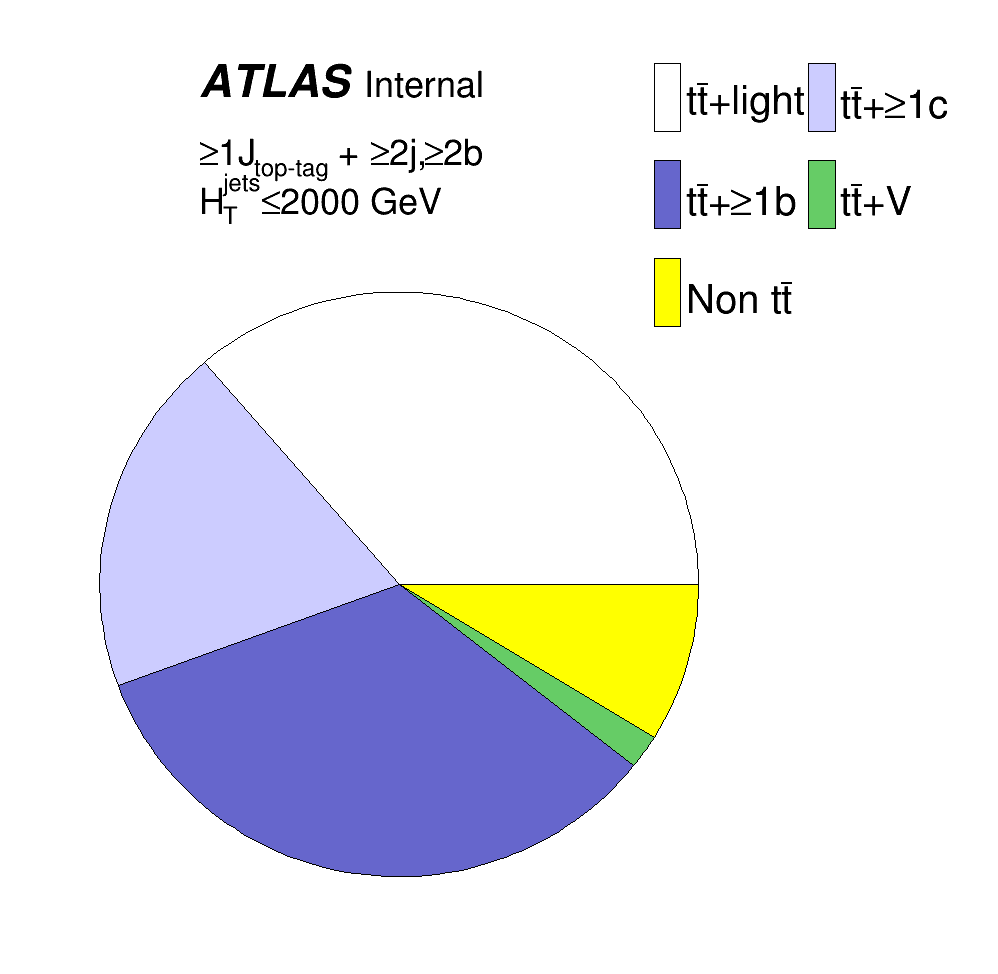
\includegraphics[keepaspectratio,scale=0.2]{images/AnalysisStrategy/PieChart_CR1_CC.png}
    \label{fig:PieChart_CR1}
  }
  \subfloat[]{
    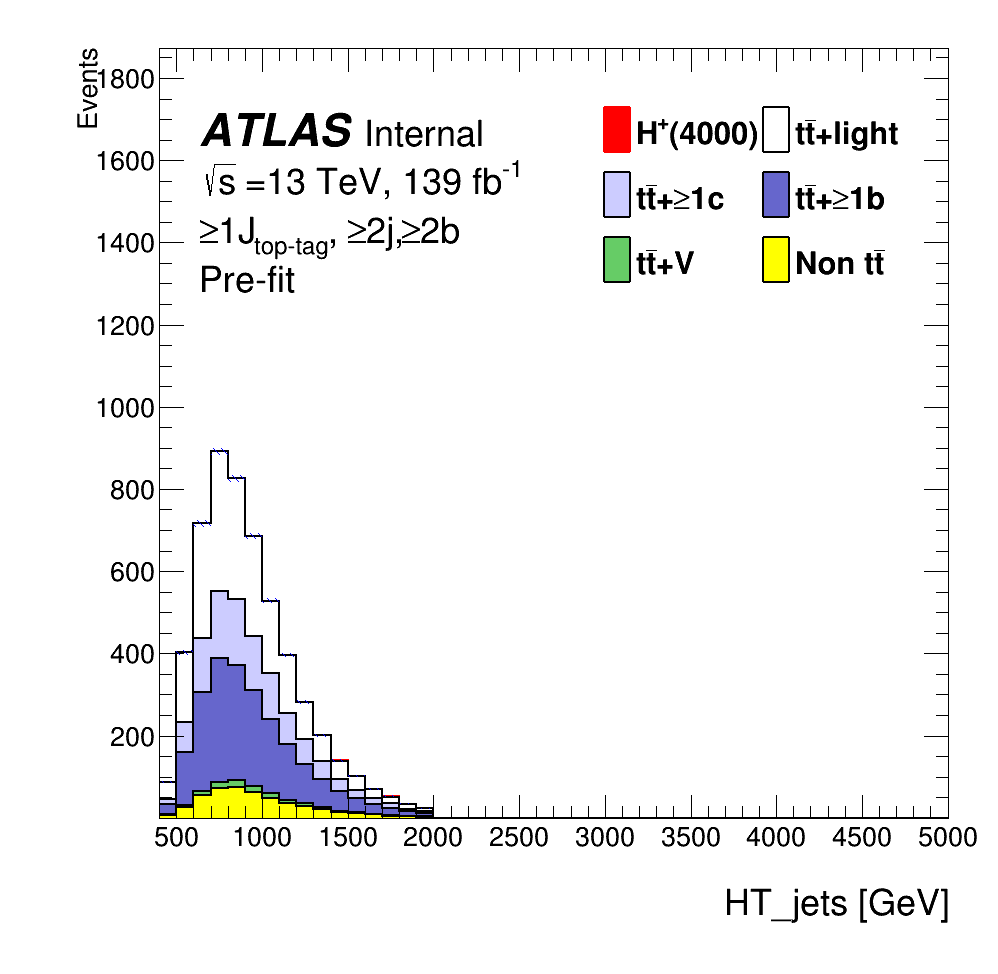
\includegraphics[keepaspectratio,scale=0.2]{images/AnalysisStrategy/HTjets_CR1_CC.png}
    \label{fig:PieChart_CR1}
  }
  \caption{Background composition in the CR1 is shown in the pie chart (a) and the $H_{\text{T}}^{\text{jets}}$ distributions (b).}
  \label{fig:BkgComposition_CR1_CC}
\end{figure}

%--- Figure for CR1
\begin{figure}[H]
  \centering
  \subfloat[]{
    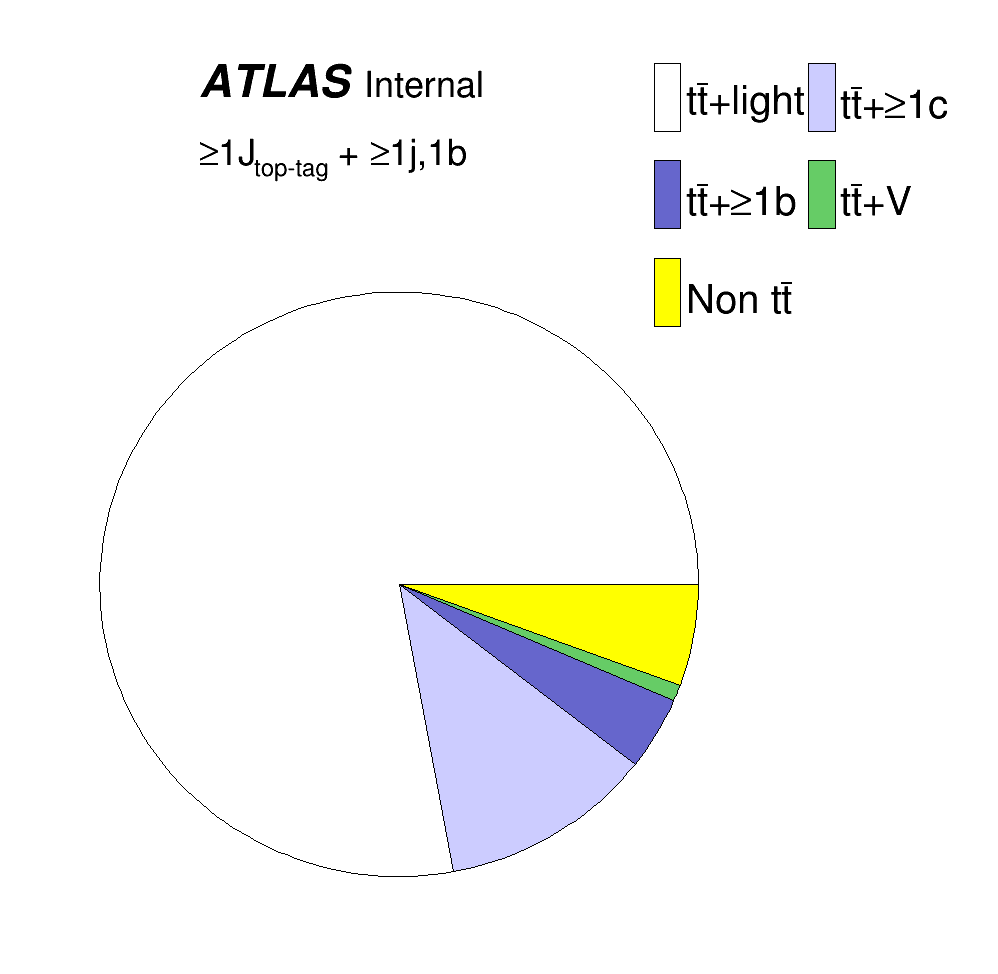
\includegraphics[keepaspectratio,scale=0.2]{images/AnalysisStrategy/PieChart_CR2_CC.png}
    \label{fig:PieChart_CR2}
  }
  \subfloat[]{
    \includegraphics[keepaspectratio,scale=0.2]{images/AnalysisStrategy/HTjets_CR2_CC.png}
    \label{fig:PieChart_CR2}
  }
  \caption{Background composition in the CR2 is shown in the pie chart (a) and the $H_{\text{T}}^{\text{jets}}$ distributions (b). The CR2 is the same region as the CR of multivariate analysis defined in Section \ref{subsubsec:RegionDefUnder3TeV}.}
  \label{fig:BkgComposition_CR2_CC}
\end{figure}

The number of expected signal and background events in the SR, CR1, and CR2 are shown in Table \ref{tab:PrefitYieldsAbove3TeV}. The predicted number of $H^{+}$ and $W'$ signal events for the 4000 and 5000 GeV mass hypothesis are estimated using $\sigma \times Br = 0.046$ pb, as done in Table \ref{tab:PrefitYields}.

\begin{table}[H]
  \centering
  \begin{tabular*}{130mm}{@{\extracolsep{\fill}}cccc}
    \hline\hline
                            & SR           & CR1             & CR2\\
    \hline
    $t\bar{t}+\text{light}$ & $22 \pm  6$  & $1928 \pm  94$  & $ 54008 \pm  2667$\\
    $t\bar{t}+\geq1c$       & $11 \pm  9$  & $1052 \pm 915$  & $  8011 \pm  1450$\\
    $t\bar{t}+\geq1b$       & $22 \pm 11$  & $1831 \pm 920$  & $  2793 \pm  1402$\\
    $t\bar{t}+W$            & $ 1 \pm  0$  & $  37 \pm   6$  & $   312 \pm    41$\\
    $t\bar{t}+Z$            & $ 1 \pm  0$  & $  67 \pm  10$  & $   294 \pm    38$\\
    $Wt$ channel            & $ 3 \pm  3$  & $ 181 \pm 104$  & $  1995 \pm   825$\\
    $t$ channel             & $ 1 \pm  0$  & $  37 \pm  24$  & $   172 \pm    56$\\
    Other top sources       & $ 1 \pm  0$  & $   8 \pm   2$  & $    34 \pm     5$\\
    $VV$, $V$+jets          & $ 5 \pm  2$  & $ 147 \pm  54$  & $  1529 \pm   530$\\
    $t\bar{t}H$             & $ 1 \pm  0$  & $ 103 \pm   4$  & $   176 \pm     5$\\
    \hline
    Total                   & $65 \pm  6$  & $5438 \pm 264$  & $ 69324 \pm  3356$\\
    \hline
    $H^{+}$ 4000 GeV        & $57 \pm 18$  & $   5 \pm   2$  & $   100 \pm    32$\\
    $H^{+}$ 5000 GeV        & $56 \pm 21$  & $   3 \pm   1$  & $    98 \pm    37$\\
    \hline\hline
  \end{tabular*}
  \caption{Number of expected and selected events split according to the SR, CR1, and CR2. The quoted uncertainties include both statistical and systematic uncertainties before fitting.}
  \label{tab:PrefitYieldsAbove3TeV}
\end{table}